\chapter{Simulações Numéricas e Discussões}

\section{Modelos elipsoidais}

As Figuras \ref{fig:triaxial}A), \ref{fig:triaxial}B), \ref{fig:triaxial}C) e \ref{fig:triaxial}D) mostram, respectivamente, as componentes $x$, $y$ e $z$ da indução magnética $\Delta \mathbf{B}(\mathbf{r})$ (Eq. \ref{eq:delta-T-tilde}) e a
anomalia de campo total $\Delta T (\mathbf{r})$ (Eq. \ref{eq:delta-T-tilde-approx}) produzidas pelo elipsoide triaxial definido de acordo com os parâmetros da Tabela \ref{tab:triaxial}.
Os dados foram calculados em uma malha de $200 \times 200$ pontos (total de 40000 pontos) localizada no plano horizontal $z = 0$ m.

\begin{table}[h]
	\begin{center}
		\begin{tabular}{|l|c|c|}
			\hline
			\textbf{Parâmetro}  & \textbf{Valor}  & \textbf{Unidade} \\
			\hline 
			$a$, $b$, $c$   & 150, 100, 75 & m\\
			\hline
			\textit{strike}   & $0$ & $^{\circ}$\\
			\hline
			\textit{dip} & $0$ & $^{\circ}$\\
			\hline
			\textit{rake} & $0$  & $^{\circ}$\\
			\hline
			$x_{c}$   & 0  & m\\
			\hline          
			$y_{c}$   & 0  & m\\
			\hline                
			$z_{c}$   & 1000 & m\\
			\hline
			$\mathbf{M}_{R}$*  & 100, $25^o$, $40^o$  & $A/m$, $^{\circ}$, $^{\circ}$\\
			\hline
			$\mathbf{B}_{0}$*    & 60000, $50^o$, $20^o$ & $nT$, $^{\circ}$, $^{\circ}$\\
			\hline
			$k_{1}$, $k_{2}$, $k_{3}$   & 0,1, 0,1, 0,1  & SI, SI, SI\\
			\hline
			Orientação das colunas da matriz $\mathbf{U}$**   & $0$, $90$, $90$  & $^{\circ}$, $^{\circ}$, $^{\circ}$\\
			\hline
		\end{tabular}
		\caption{Parâmetros do elipsoide triaxial modelado. *Valores de intensidade, inclinação e declinação respectivamente. **Ângulo de \textit{strike} , \textit{dip}  e \textit{rake} , respectivamente, para calcular os vetores unitários $\mathbf{u}_{1}$, $\mathbf{u}_{2}$, $\mathbf{u}_{3}$ por meio das Eqs. \ref{eq:v1_triaxial_prolate}, \ref{eq:v2_triaxial_prolate} e \ref{eq:v3_triaxial_prolate}.}
	\end{center}
	\label{tab:triaxial}
\end{table}

\begin{figure}[hbt!]
	\centering 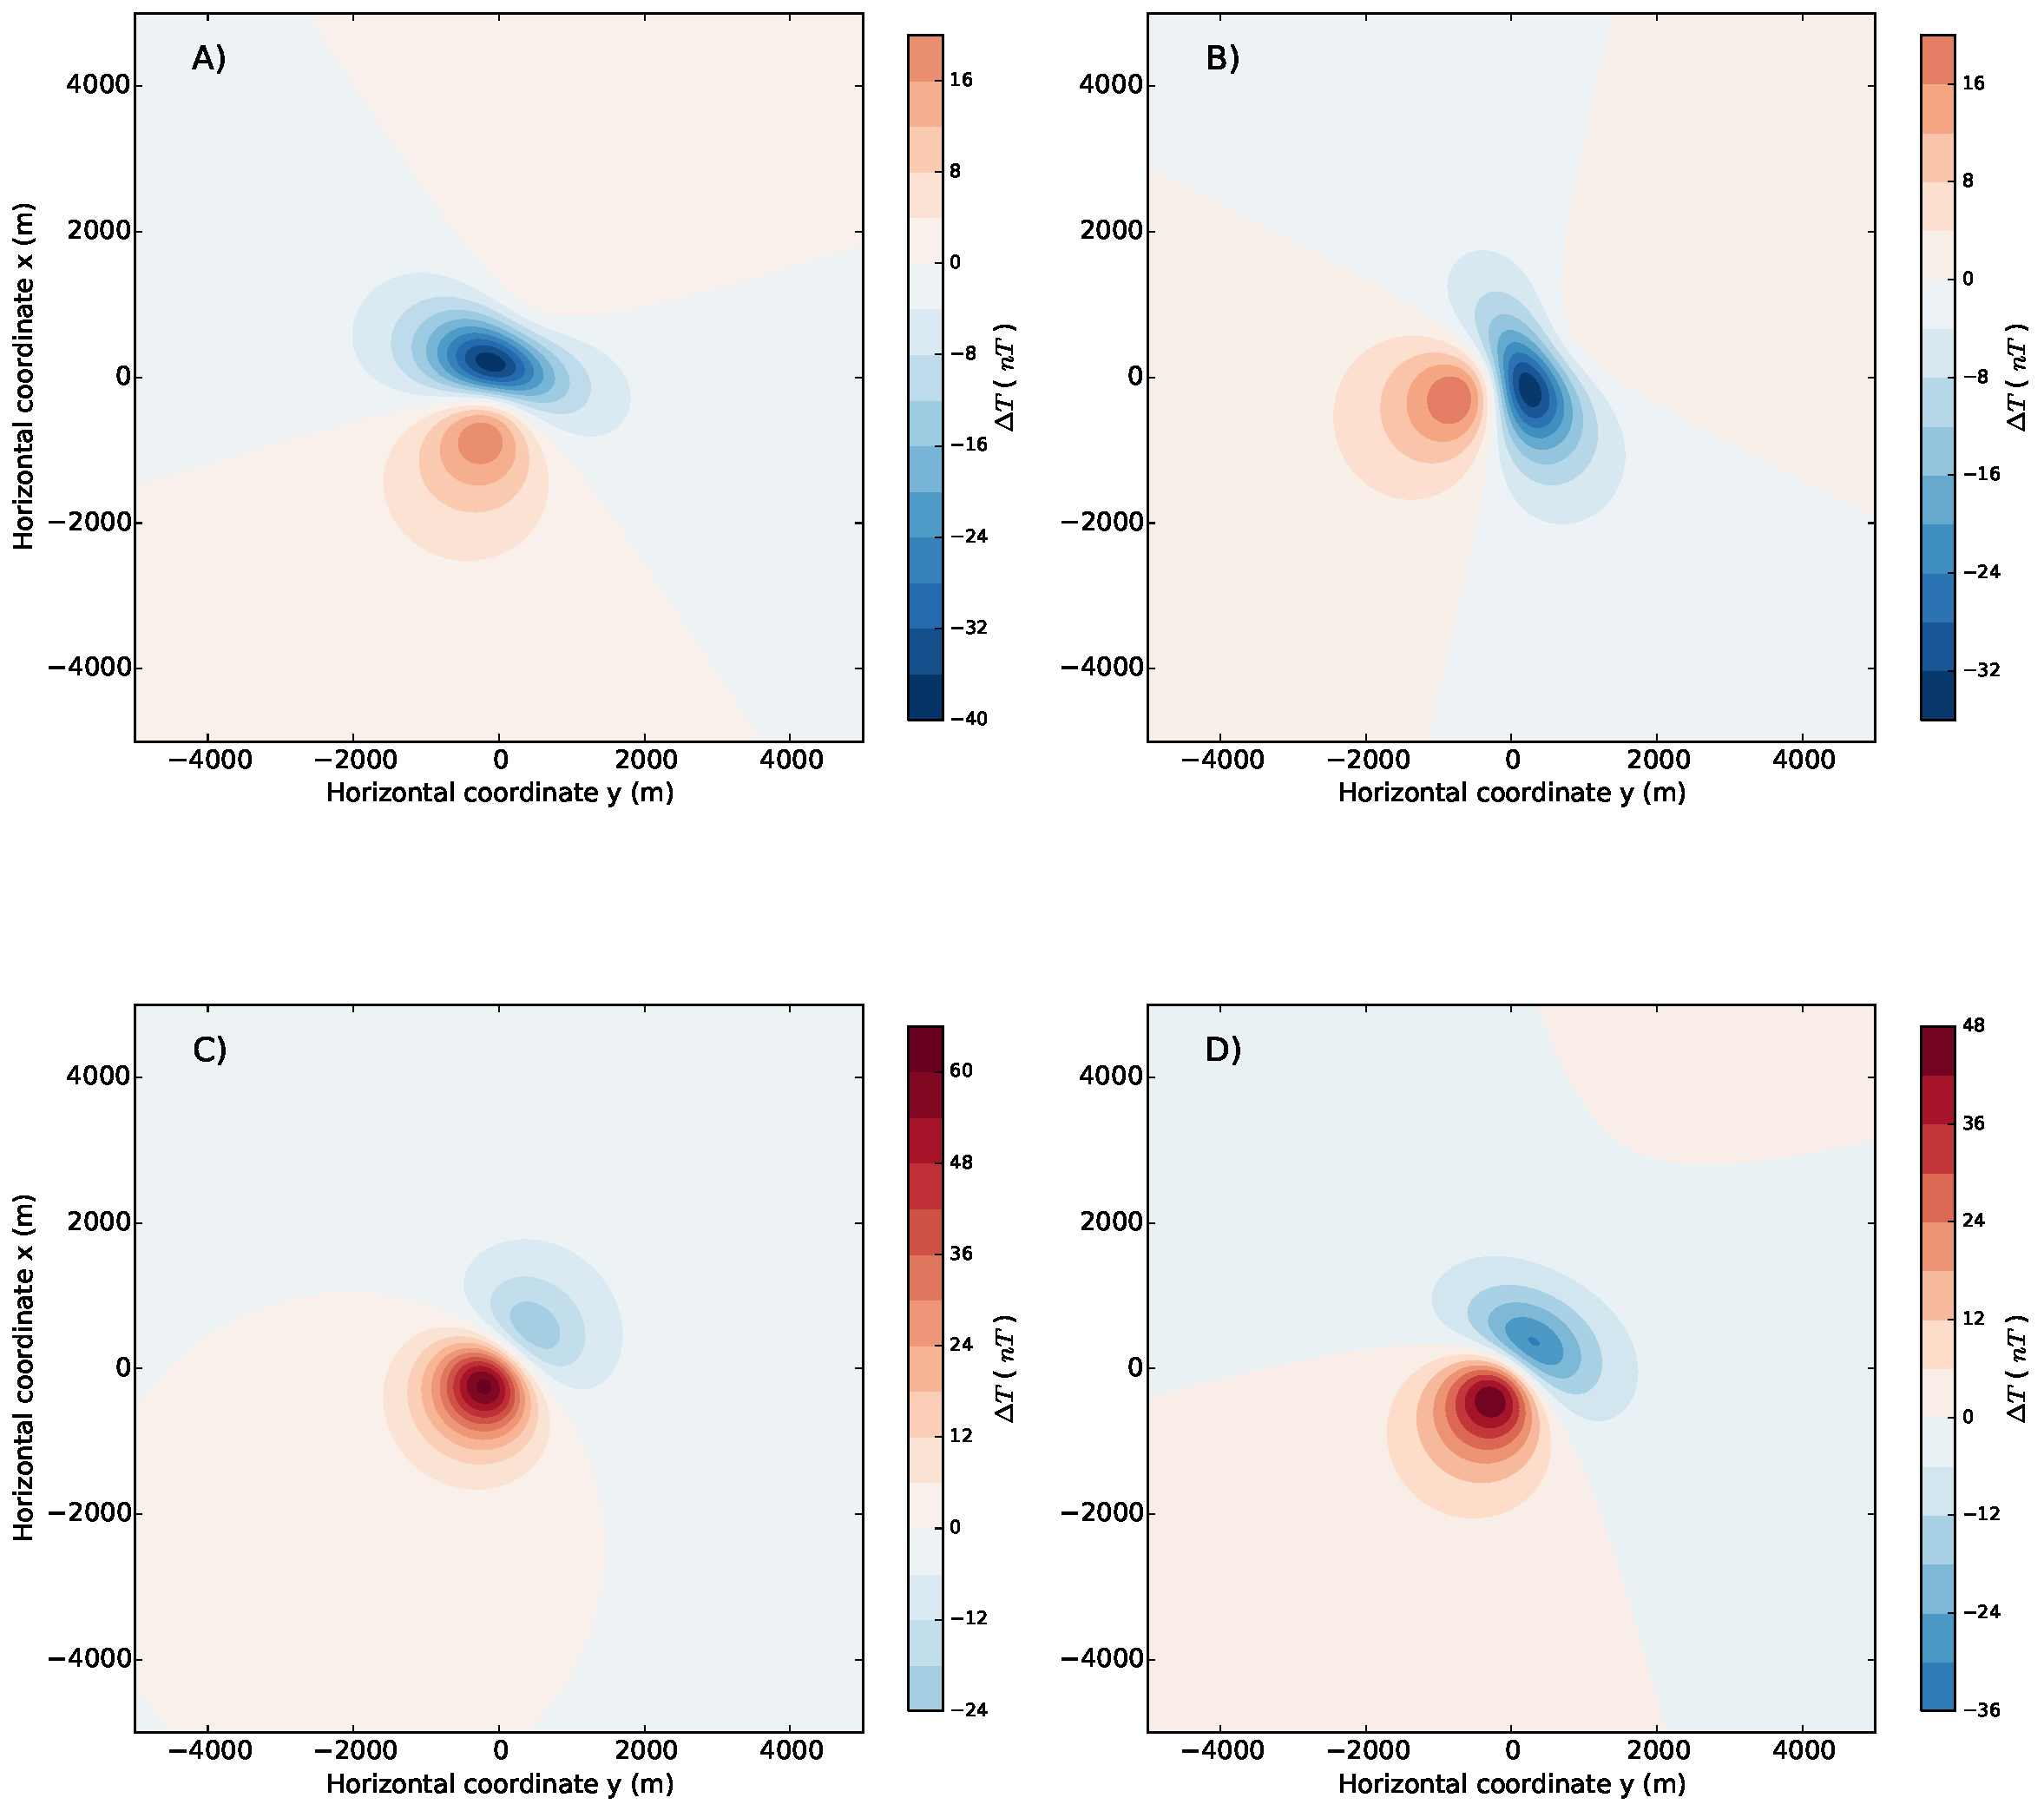
\includegraphics[width=16cm,height=16cm]{figures/ellipsoid_triaxial}
	\caption[Campo gerado pelo elipsoide triaxial definido na Tabela \ref{tab:triaxial}. A), B) e C) Componentes $x$, $y$ e $z$, respectivamente, da indução magnética $\Delta \mathbf{B}(\mathbf{r})$ (Eq. \ref{eq:delta-T-tilde}). D) Anomalia de campo total $\Delta T (\mathbf{r})$ (Eq. \ref{eq:delta-T-tilde-approx}). Todos os valores estão em nT.]{Campo gerado pelo elipsoide triaxial definido na Tabela \ref{tab:triaxial}. A), B) e C) Componentes $x$, $y$ e $z$, respectivamente, da indução magnética $\Delta \mathbf{B}(\mathbf{r})$ (Eq. \ref{eq:delta-T-tilde}). D) Anomalia de campo total $\Delta T (\mathbf{r})$ (Eq. \ref{eq:delta-T-tilde-approx}). Todos os valores estão em nT.}
	\label{fig:triaxial}
\end{figure}

As Figuras \ref{fig:prolate}A), \ref{fig:prolate}B), \ref{fig:prolate}C) e \ref{fig:prolate}D) mostram, respectivamente, as componentes $x$, $y$ e $z$ da indução magnética $\Delta \mathbf{B}(\mathbf{r})$ (Eq. \ref{eq:delta-T-tilde}) e a
anomalia de campo total $\Delta T (\mathbf{r})$ (Eq. \ref{eq:delta-T-tilde-approx}) produzidas pelo elipsoide prolato definido de acordo com os parâmetros da Tabela 4.2.

As Figuras \ref{fig:oblate}A), \ref{fig:oblate}B), \ref{fig:oblate}C) e \ref{fig:oblate}D) mostram, respectivamente, as componentes $x$, $y$ e $z$ da indução magnética $\Delta \mathbf{B}(\mathbf{r})$ (Eq. \ref{eq:delta-T-tilde}) e a
anomalia de campo total $\Delta T (\mathbf{r})$ (Eq. \ref{eq:delta-T-tilde-approx}) produzidas pelo elipsoide prolato definido de acordo com os parâmetros da Tabela 4.3.
\\\\\\

\begin{table}[h!]
	\begin{center}
		\begin{tabular}{|l|c|c|}
			\hline
			\textbf{Parâmetro}  & \textbf{Valor}  & \textbf{Unidade} \\
			\hline 
			$a$, $b$   & 200, 100 & m\\
			\hline
			\textit{strike}   & $45$ & $^{\circ}$\\
			\hline
			\textit{dip}    & $0$ & $^{\circ}$\\
			\hline
			\textit{rake}   & $0$  & $^{\circ}$\\
			\hline
			$x_c$   & 0  & m\\
			\hline          
			$y_c$   & 0  & m\\
			\hline                
			$z_c$   & 1000  & m\\
			\hline
			$\mathbf{M}_{R}$*  & 100, $90$, $0$ & $A/m$, $^{\circ}$, $^{\circ}$\\
			\hline
			$\mathbf{B}_{0}$*    & 60000, $50$, $20$ & $nT$, $^{\circ}$, $^{\circ}$\\
			\hline
			$k_{1}$, $k_{2}$, $k_{3}$   & 0,1, 0,1, 0,1  & SI, SI, SI\\
			\hline
			Orientação das colunas da matriz $\mathbf{U}$**   & $0$, $90$, $90$  & $^{\circ}$, $^{\circ}$, $^{\circ}$\\
			\hline
			
		\end{tabular}
		\caption{Parâmetros do elipsoide prolato modelado. *Valores de intensidade, inclinação e declinação respectivamente. **Ângulo de \textit{strike} , \textit{dip}  e \textit{rake} , respectivamente, para calcular os vetores unitários $\mathbf{u}_{1}$, $\mathbf{u}_{2}$, $\mathbf{u}_{3}$ por meio das Eqs. \ref{eq:v1_triaxial_prolate}, \ref{eq:v2_triaxial_prolate} e \ref{eq:v3_triaxial_prolate}.}
	\end{center}
	\label{tab:prolato}
\end{table}

\begin{table}[h!]
	\begin{center}
		\begin{tabular}{lc}
		
			 &  \\
			 & \\
			 & \\
			 & \\
			& \\
			& \\ 
			& \\
			& \\
			& \\ 
			& \\
\end{tabular}
\end{center}
\end{table}

\begin{table}[h!]
	\begin{center}
		\begin{tabular}{|l|c|c|}
			\hline
			\textbf{Parâmetro}  & \textbf{Valor} & \textbf{Unidade} \\
			\hline 
			$a$, $b$  & 100, 200 & m \\
			\hline
			\textit{strike}   & $45$ &  $^{\circ}$\\
			\hline
			\textit{dip}    & $0$ &  $^{\circ}$\\
			\hline
			\textit{rake}   & $0$  &  $^{\circ}$\\
			\hline
			$x_c $  & 0  & m\\
			\hline          
			$y_c$   & 0  & m\\
			\hline                
			$z_c$   & 1000  & m\\
			\hline
			$\mathbf{M}_{R}$*  & 100, $90$, $0$  & $A/m$, $^{\circ}$, $^{\circ}$\\
			\hline
			$\mathbf{B}_{0}$*    & 60000, $50$, $20$ & $nT$, $^{\circ}$, $^{\circ}$\\
			\hline
			$k_{1}$, $k_{2}$, $k_{3}$   & 0,1, 0,1, 0,1  & SI, SI, SI\\
			\hline
			Orientação das colunas da matriz $\mathbf{U}$**   & $0$, $90$, $90$  &  $^{\circ}$,  $^{\circ}$,  $^{\circ}$\\
			\hline
		\end{tabular}
		\caption{Parâmetros do elipsoide oblato modelado. *Valores de intensidade, inclinação e declinação respectivamente. **Ângulo de \textit{strike} , \textit{dip}  e \textit{rake} , respectivamente, para calcular os vetores unitários $\mathbf{u}_{1}$, $\mathbf{u}_{2}$, $\mathbf{u}_{3}$ por meio das Eqs. \ref{eq:v1_oblate}, \ref{eq:v2_oblate} e \ref{eq:v3_oblate}.}
	\end{center}
	\label{tab:oblate}
\end{table}

\begin{figure}[hbt!]
	\centering 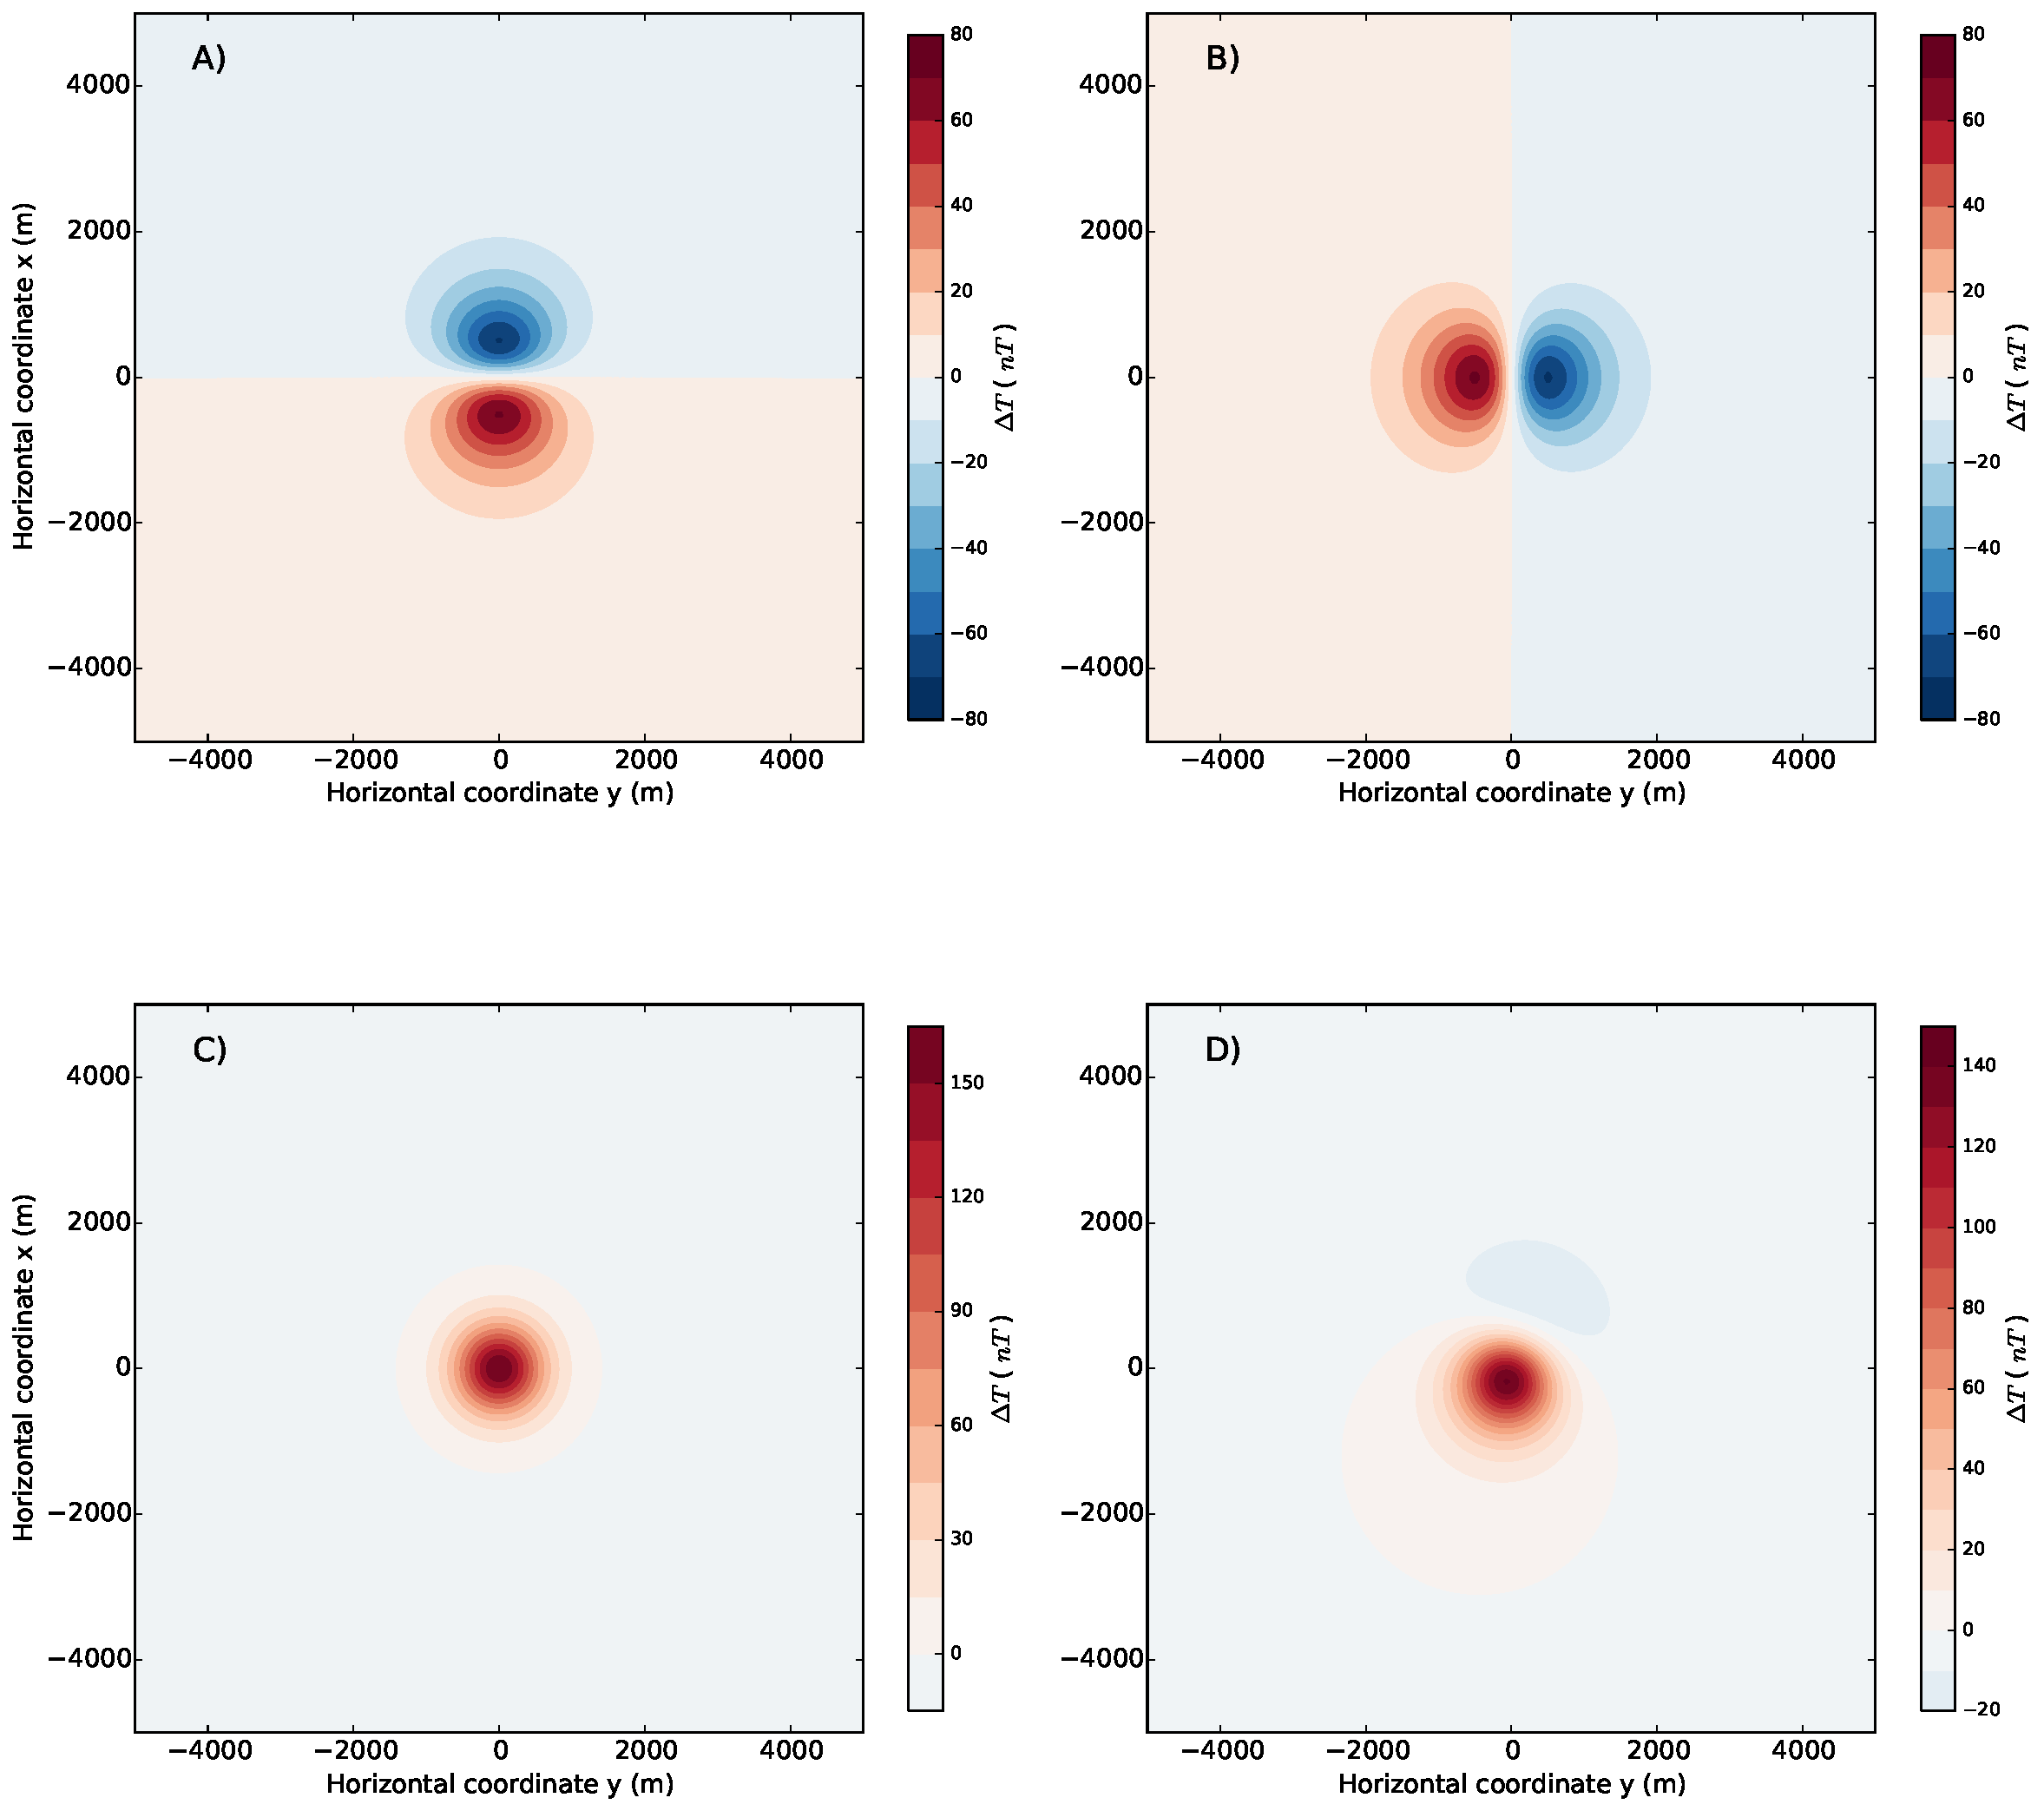
\includegraphics[width=16cm,height=16cm]{figures/ellipsoid_prolate}
	\caption[As componentes do campo magnético gerado por um elipsoide prolato e a anomalia de campo total aproximada.]{As componentes 
		do campo magnético gerado por um elipsoide prolato de parâmetros conforme a tabela 4.2 e a anomalia de campo total aproximada. Em A) a componente Bx do campo, em B) a componente By, em C) a componente Bz e em D) a anomalia de campo total aproximada.}
	\label{fig:prolate}
\end{figure}

\begin{table}[h!]
	\begin{center}
		\begin{tabular}{lc}
			
			&  \\
			& \\
			& \\
			& \\
			& \\
			& \\ 
			& \\
			& \\
		\end{tabular}
	\end{center}
\end{table}

\begin{figure}[hbt!]
	\centering 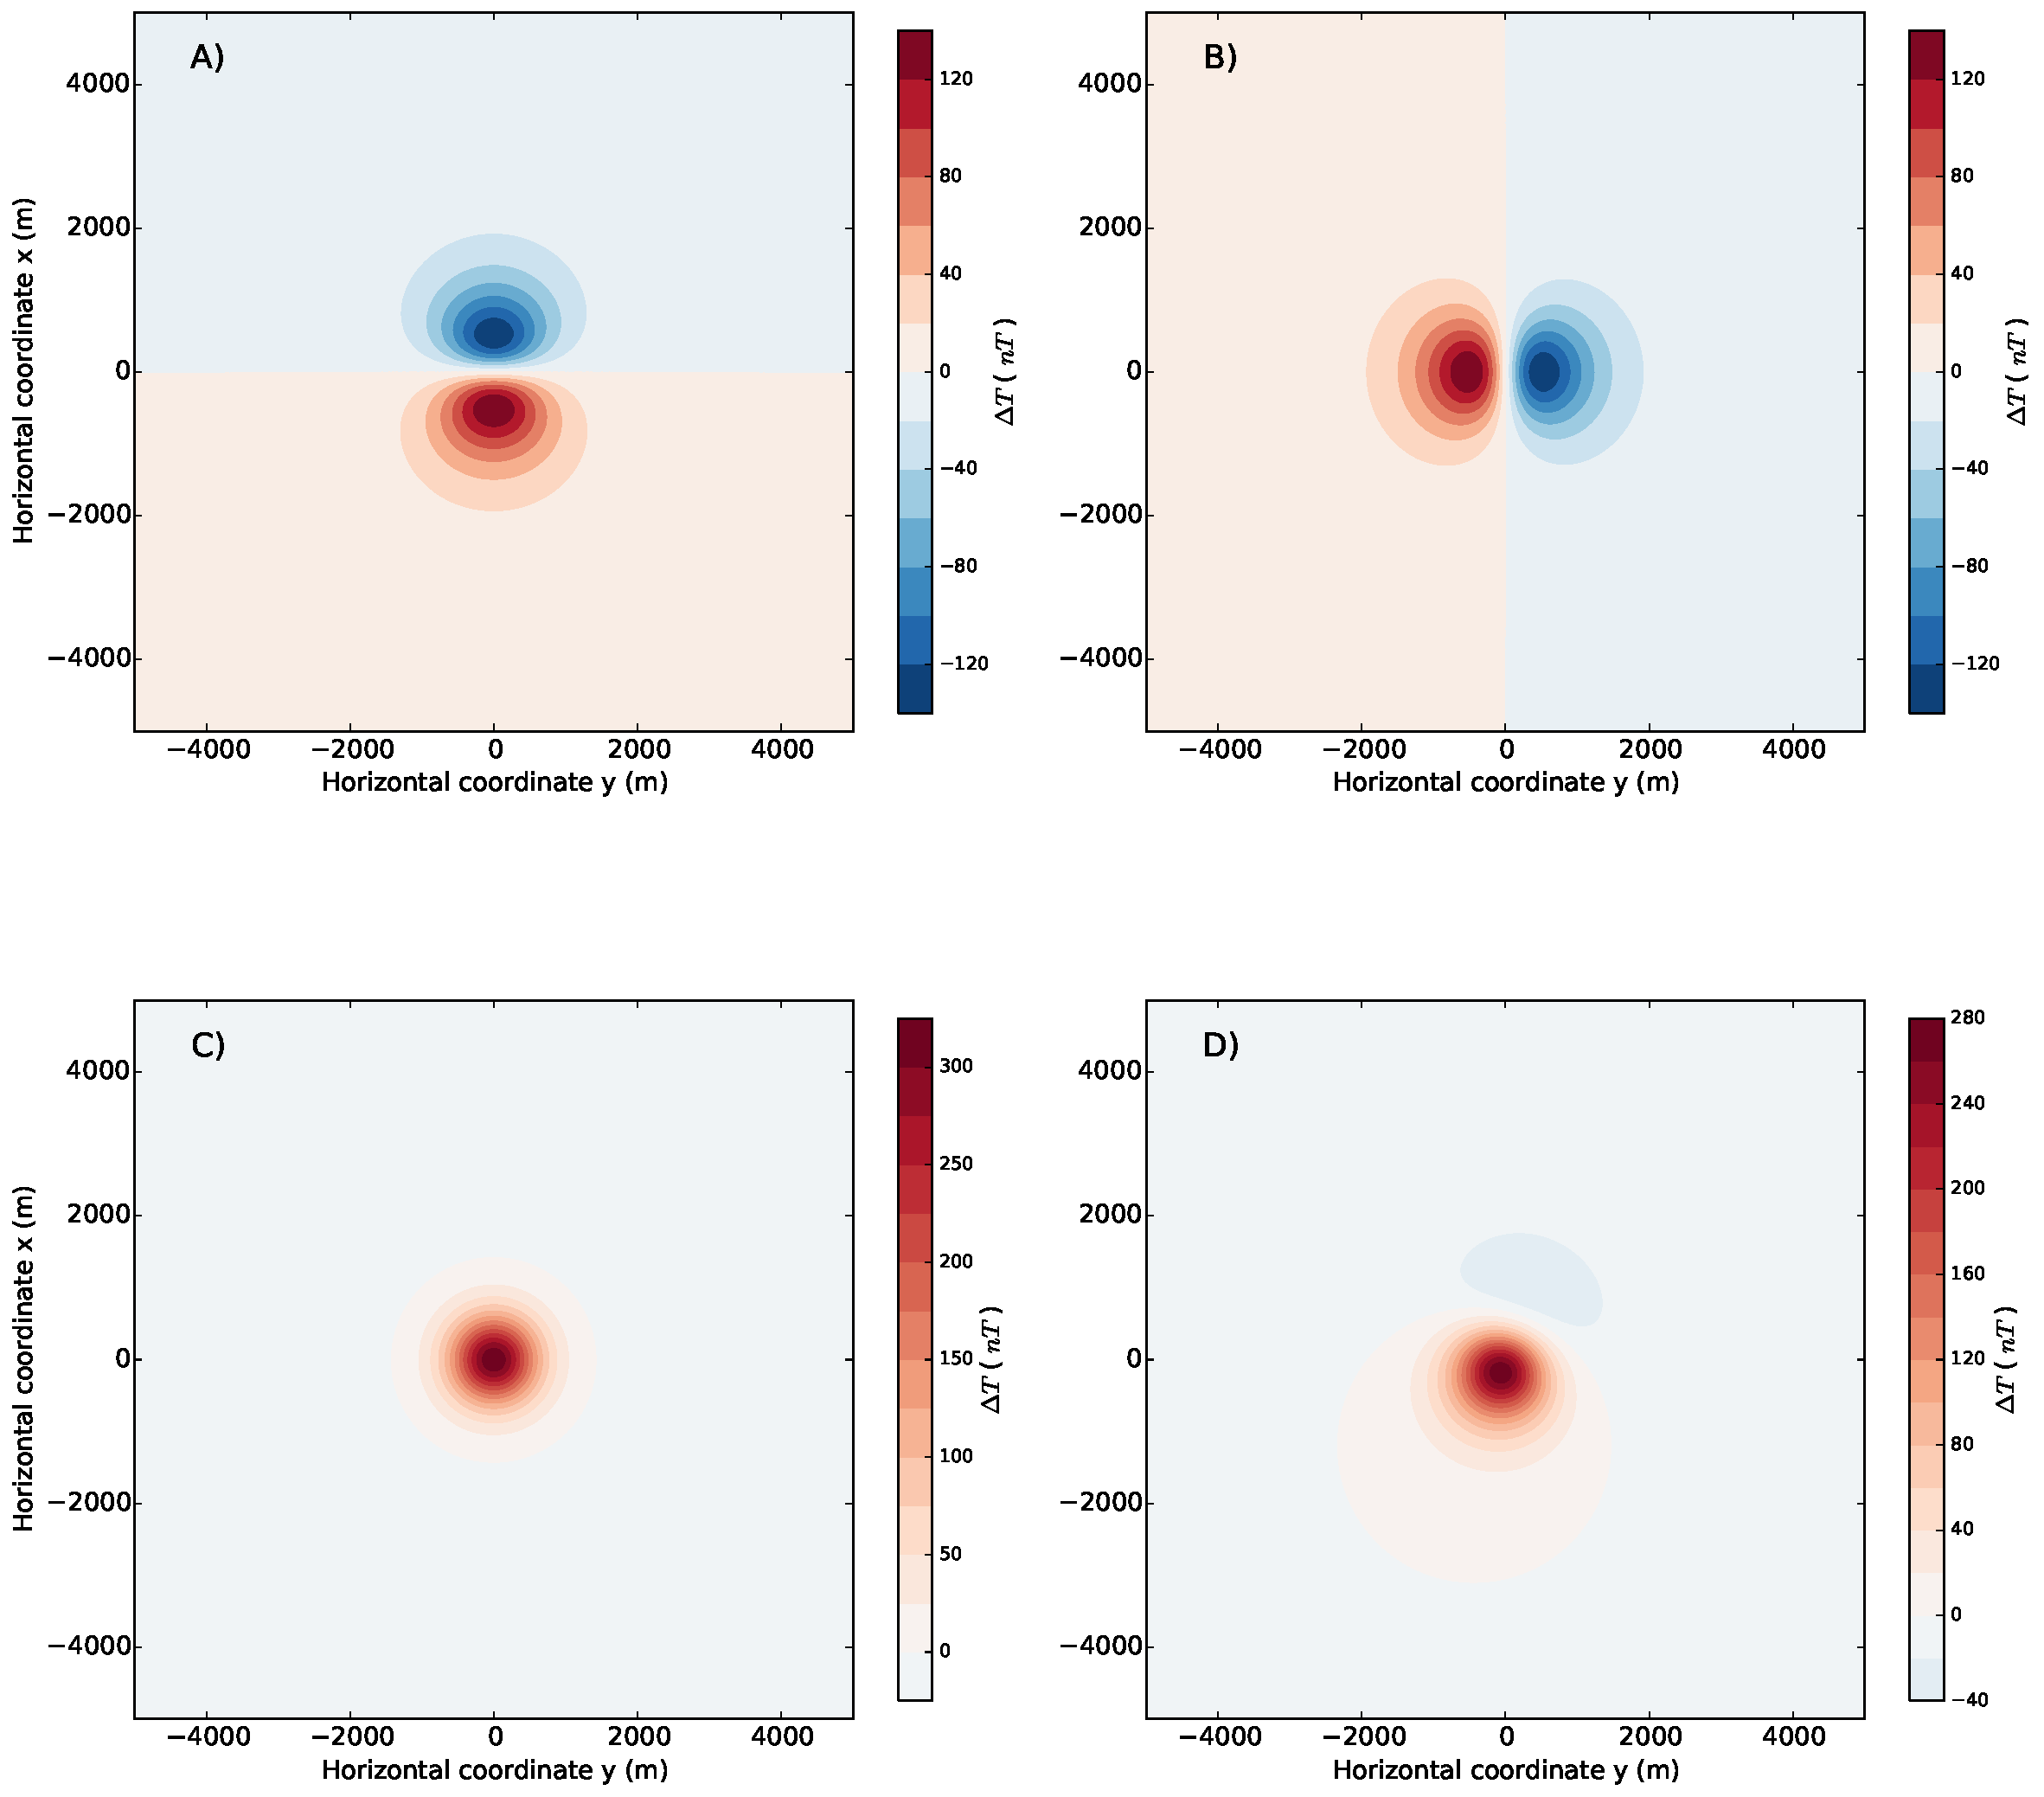
\includegraphics[width=16cm,height=16cm]{figures/ellipsoid_oblate}
	\caption[As componentes do campo magnético gerado por um elipsoide oblato e a anomalia de campo total aproximada.]{As componentes 
		do campo magnético gerado por um elipsoide oblato de parâmetros conforme a tabela 4.3 e a anomalia de campo total aproximada. Em A) a componente Bx do campo, em B) a componente By, em C) a componente Bz e em D) a anomalia de campo total aproximada.}
	\label{fig:oblate}
\end{figure}

As Figuras \ref{fig:ellipsoid_triaxial_multi}A), \ref{fig:ellipsoid_triaxial_multi}B), \ref{fig:ellipsoid_triaxial_multi}C) e \ref{fig:ellipsoid_triaxial_multi}D) mostram, respectivamente, as componentes $x$, $y$ e $z$ da indução magnética $\Delta \mathbf{B}(\mathbf{r})$ (Eq. \ref{eq:delta-T-tilde}) e a
anomalia de campo total $\Delta T (\mathbf{r})$ (Eq. \ref{eq:delta-T-tilde-approx}) produzidas por dois elipsoides triaxiais definidos de acordo com os parâmetros da Tabela 4.4.

\begin{table}[h!]
	\begin{center}
		\begin{tabular}{lc}
			
			&  \\
			&  \\
			&  \\
			&  \\
		\end{tabular}
	\end{center}
\end{table}

\begin{table}[h!]
	\begin{center}
		\begin{tabular}{|l|c|c|}
			\hline
			\textbf{Parâmetro}  & \textbf{Valor}  & \textbf{Unidade}\\
			\hline 
			$a$, $b$, $c$   & 150, 100, 75 & m\\
			\hline
			\textit{strike}   & $0$ & $^{\circ}$\\
			\hline
			\textit{dip}    & $0$ & $^{\circ}$\\
			\hline
			\textit{rake}   & $0$  & $^{\circ}$\\
			\hline
			$x_c$   & -2500  & m\\
			\hline          
			$y_c$   & -2500  & m\\
			\hline                
			$z_c$  & 1000  & m\\
			\hline
			$\mathbf{M}_{R}$*  & 100, $25^o$, $40^o$  & $A/m$, $^{\circ}$, $^{\circ}$\\
			\hline
			$k_1$, $k_2$, $k_3$   & 0,1, 0,1, 0,1  & SI, SI, SI\\
			\hline
			Orientação das colunas da matriz $\mathbf{U}$**   & $0$, $90$, $90$  & $^{\circ}$, $^{\circ}$, $^{\circ}$\\
			\hline 
			$a_2$, $b_2$, $c_2$   & 200, 120, 60 & m\\
			\hline
			\textit{strike}$_2$   & $0$ & $^{\circ}$\\
			\hline
			\textit{dip}$_2$    & $0$ & $^{\circ}$\\
			\hline
			\textit{rake}$_2$   & $0$  & $^{\circ}$\\
			\hline
			$x_{c2}$   & 2500  & m\\
			\hline          
			$y_{c2}$   & 2500  & m\\
			\hline                
			$z_{c2}$   & 1000  & m\\
			\hline
			$\mathbf{M}_{R2}$*  & 75, $25^o$, $40^o$  & $A/m$, $^{\circ}$, $^{\circ}$\\
			\hline
			$k_12$, $k_22$, $k_32$   & 0,1, 0,1, 0,1  & SI, SI, SI\\
			\hline
			Orientação das colunas da matriz $\mathbf{U}_2$**   & $0$, $90$, $90$  & $^{\circ}$, $^{\circ}$, $^{\circ}$\\
			\hline
			$\mathbf{B}_{0}$*    & 60000, $50^o$, $20^o$ & $nT$, $^{\circ}$, $^{\circ}$\\
			\hline			
		\end{tabular}
		\caption{Parâmetros dos  dois elipsoides triaxiais modelados. *Valores de intensidade, inclinação e declinação respectivamente. **Ângulo de \textit{strike} , \textit{dip}  e \textit{rake} , respectivamente, para calcular os vetores unitários $\mathbf{u}_{1}$, $\mathbf{u}_{2}$, $\mathbf{u}_{3}$ por meio das Eqs. \ref{eq:v1_triaxial_prolate}, \ref{eq:v2_triaxial_prolate} e \ref{eq:v3_triaxial_prolate}.}
	\end{center}
	\label{tab:ellipsoid_triaxial_multi}
\end{table}

\begin{table}[h!]
	\begin{center}
		\begin{tabular}{lc}
			
			&  \\
			& \\
			& \\
			& \\
			& \\
			& \\ 
			& \\
			& \\
				& \\
				& \\ 
				& \\
		\end{tabular}
	\end{center}
\end{table}

\begin{figure}[hbt!]
	\centering 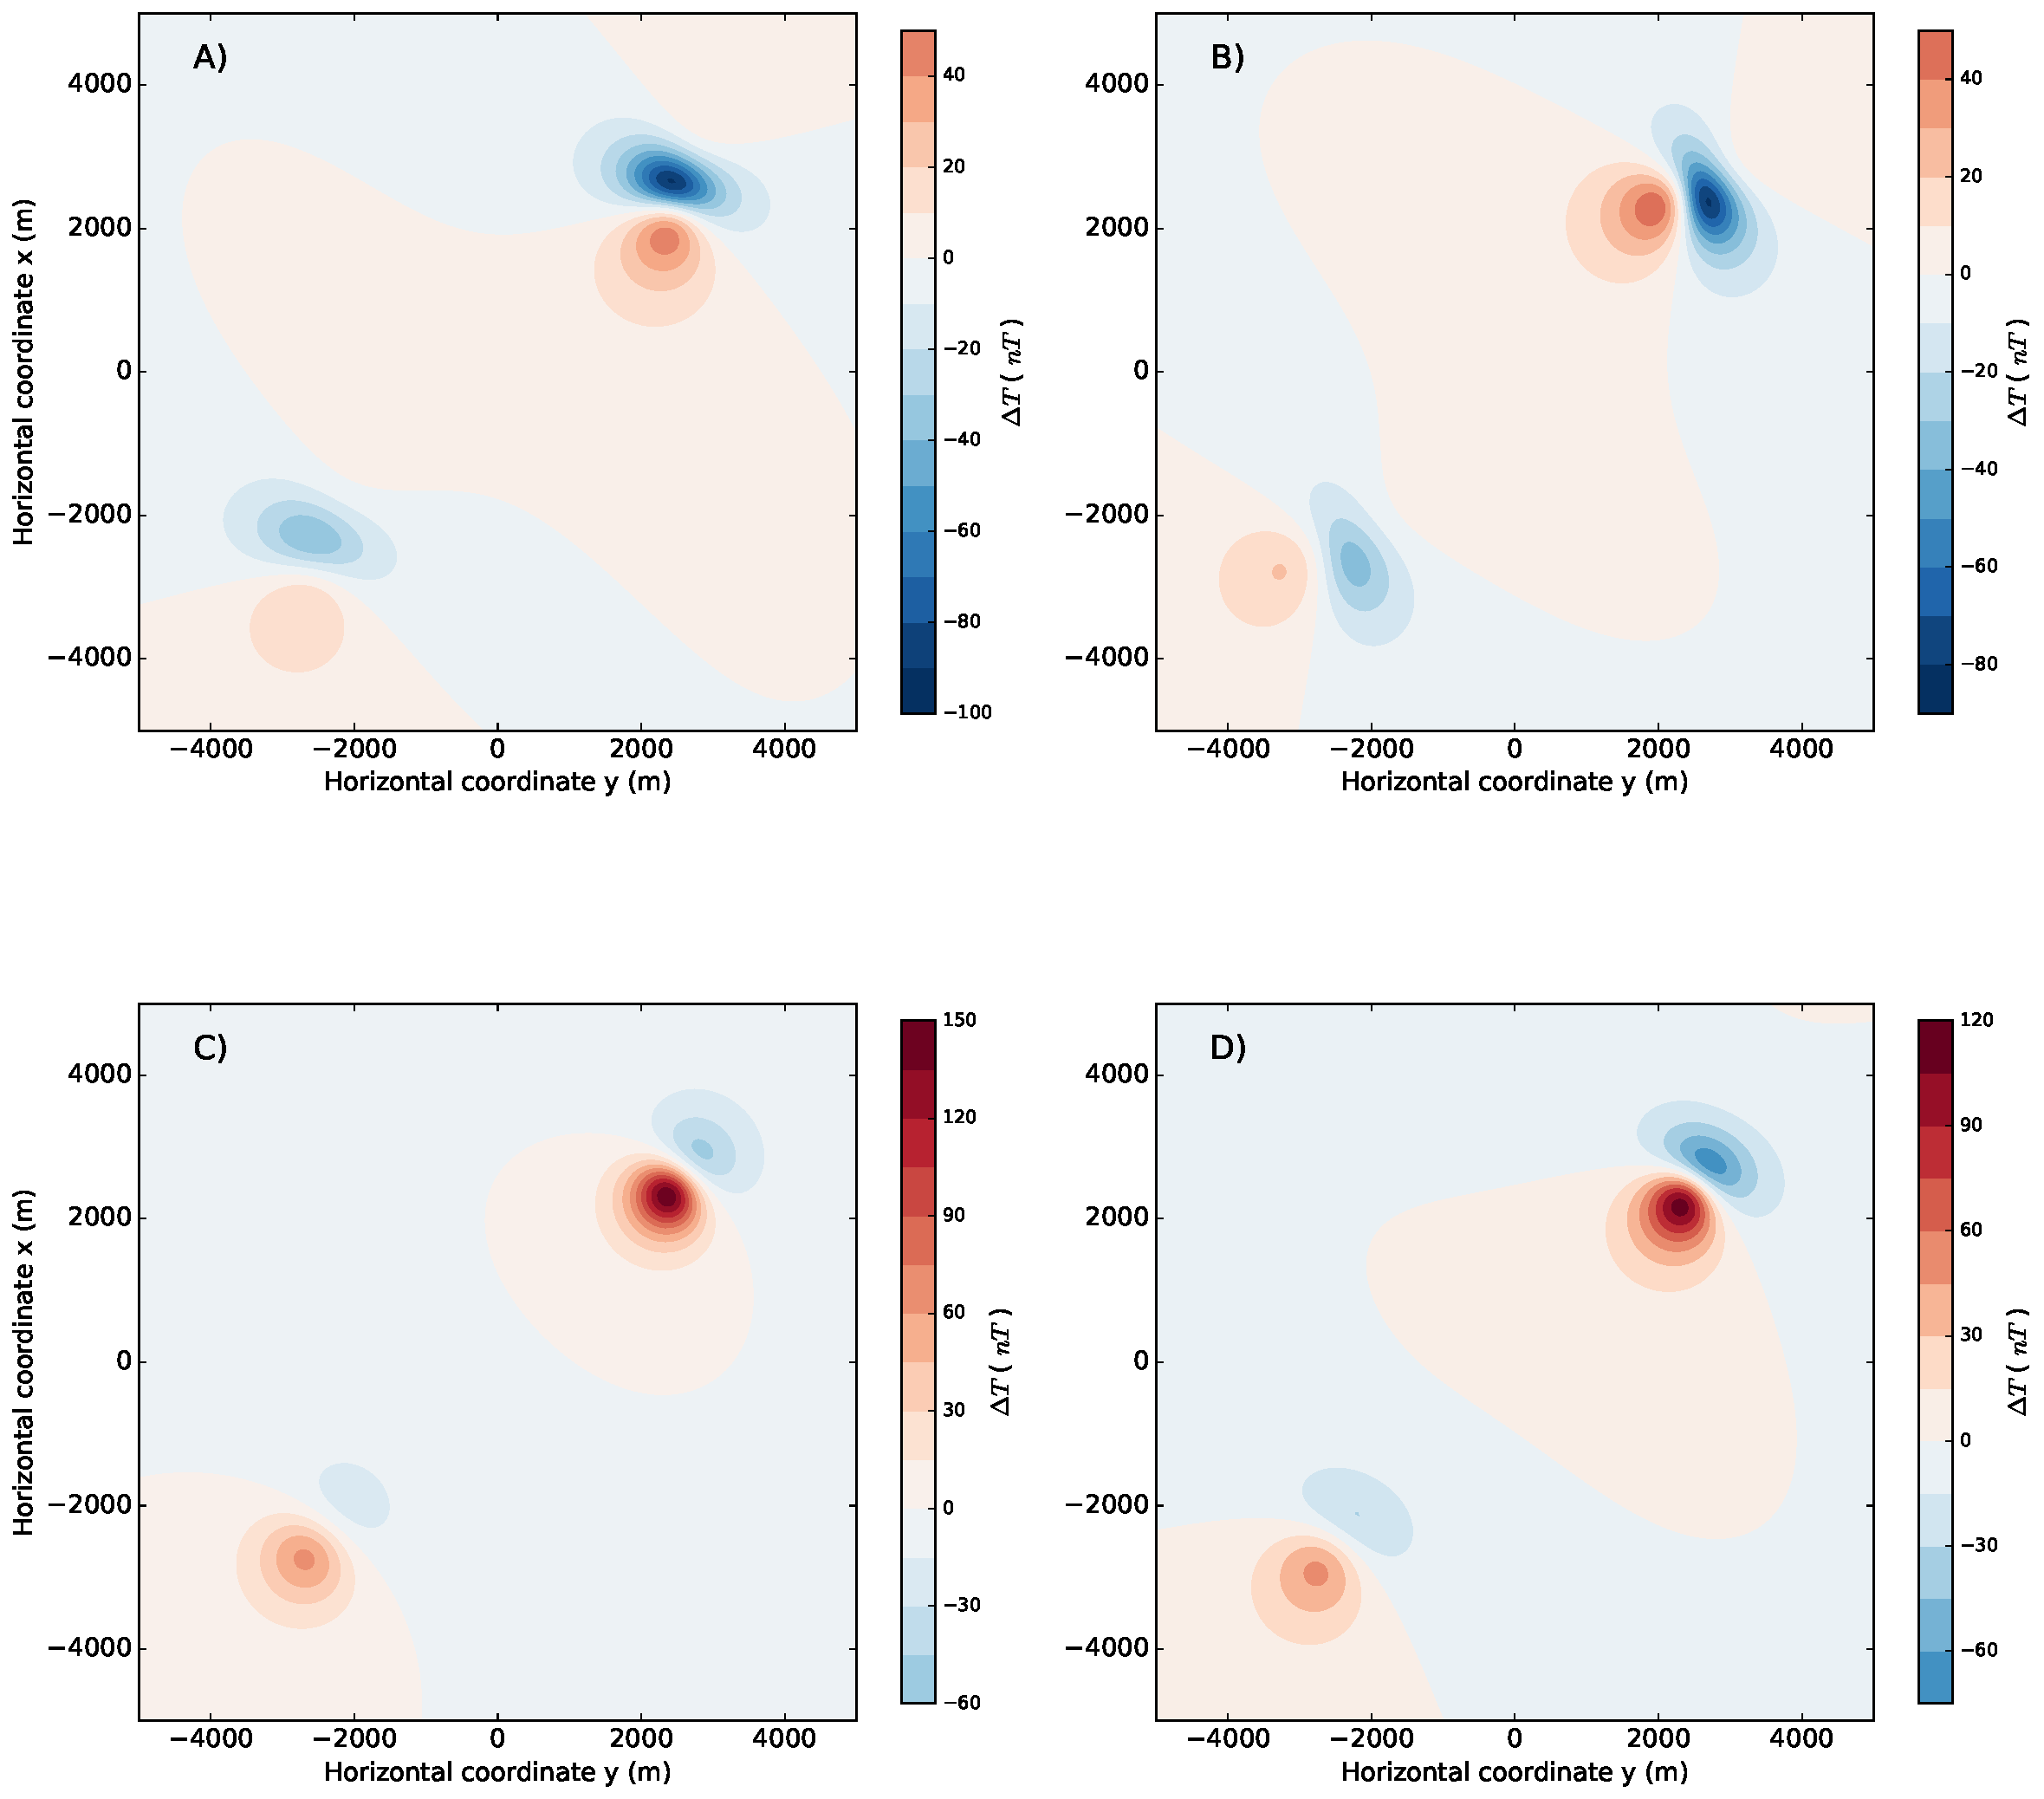
\includegraphics[width=16cm,height=16cm]{figures/ellipsoid_triaxial_multi}
	\caption[As componentes do campo magnético gerado por dois corpos triaxiais e a anomalia de campo total aproximada.]{As componentes 
		do campo magnético gerado pelos elipsoides triaxiais de parâmetros conforme a tabela 4.4 e a anomalia de campo total aproximada. Em A) a componente Bx do campo, em B) a componente By, em C) a componente Bz e em D) a anomalia de campo total aproximada.}
	\label{fig:ellipsoid_triaxial_multi}
\end{figure}


\begin{figure}[hbt!]
	\centering 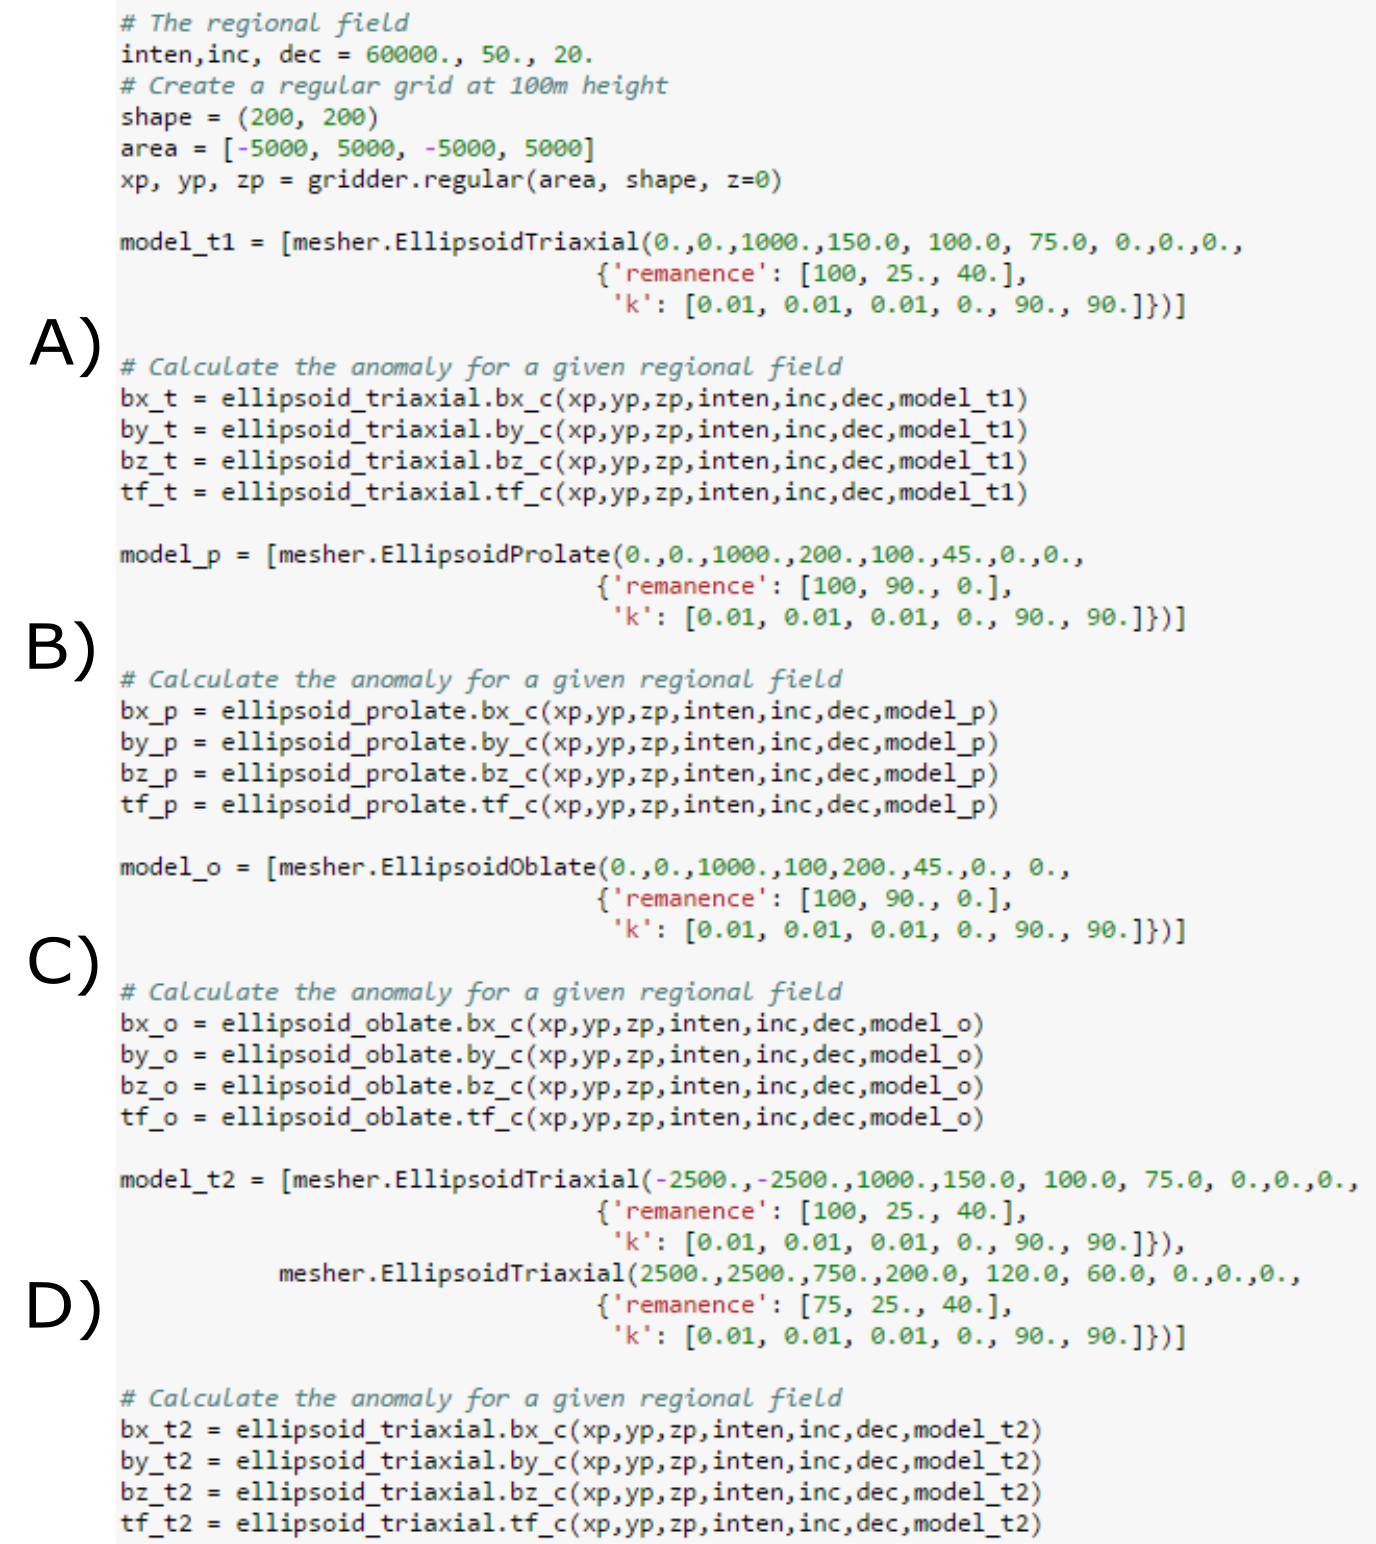
\includegraphics[width=16 cm,height=20 cm]{figures/mag_fields_01}
	\caption[\textit{Scripts} utilizados para gerar os resultados mostrados: A) na Figura \ref{fig:triaxial}, B) na Figura\ref{fig:prolate}, C) na Figura \ref{fig:oblate} e D) na Figura \ref{fig:ellipsoid_triaxial_multi}. A descrição do código é similar àquela mostrada na Figura \ref{fig:Cookbook_Triaxial}.]{\textit{Scripts} utilizados para gerar os resultados mostrados: A) na Figura \ref{fig:triaxial}, B) na Figura\ref{fig:prolate}, C) na Figura \ref{fig:oblate} e D) na Figura \ref{fig:ellipsoid_triaxial_multi}. A descrição do código é similar àquela mostrada na Figura \ref{fig:Cookbook_Triaxial}.}
	\label{fig:mag_fields_0}
\end{figure}

\begin{table}[h!]
	\begin{center}
		\begin{tabular}{lc}
			
			&  \\
			& \\
			& \\
			& \\
			& \\
			& \\ 
			& \\
			& \\
		\end{tabular}
	\end{center}
\end{table}

\section{Fatores de desmagnetização}

Os fatores de desmagnetização são importantíssimos para a modelagem de corpos com alta susceptibilidade e dependem apenas da sua forma geométrica no modelo elipsoidal. 

Na Figura \ref{fig:n_triaxial} observamos o comportamento afastado destes elementos, quando os semi-eixos de elipsoide triaxial possuem tamanhos diferentes, e a tendência de se aproximarem para um mesmo valor quando possuem valores próximos (se aproximando de uma esfera, que possui o valor de $1/3$ no SI para todos os elementos dos fatores de desmagnetização). Para tal, simulamos um elipsoide triaxial inicialmente com semi-eixos $a_0=500$ m, $b_0=100$ m e $c_0=50$ m e o usamos como referência para gerar 200 outros elipsoides triaxiais calculando seus fatores de desmagnetização $\tilde{n}^{\dagger}_{11}$, $\tilde{n}^{\dagger}_{22}$ e $\tilde{n}^{\dagger}_{33}$ pelas Eq. \ref{eq:n-tilde-dagger-11-triaxial}, \ref{eq:n-tilde-dagger-22-triaxial} e \ref{eq:n-tilde-dagger-33-triaxial}. Os sei-exis destes 100 elipsoides são dados por $a=a_0+u$, $b=b_0+u$ e $c=c_0+u$, em que $500 \le u \ge 30000$. Ou seja, os semi-eixos aumentam igualmente por uma variável $u$ crescente e quanto maior essa variável, mais esféricos serão os elipsoides obtidos.


\begin{figure}[hbt!]
	\centering 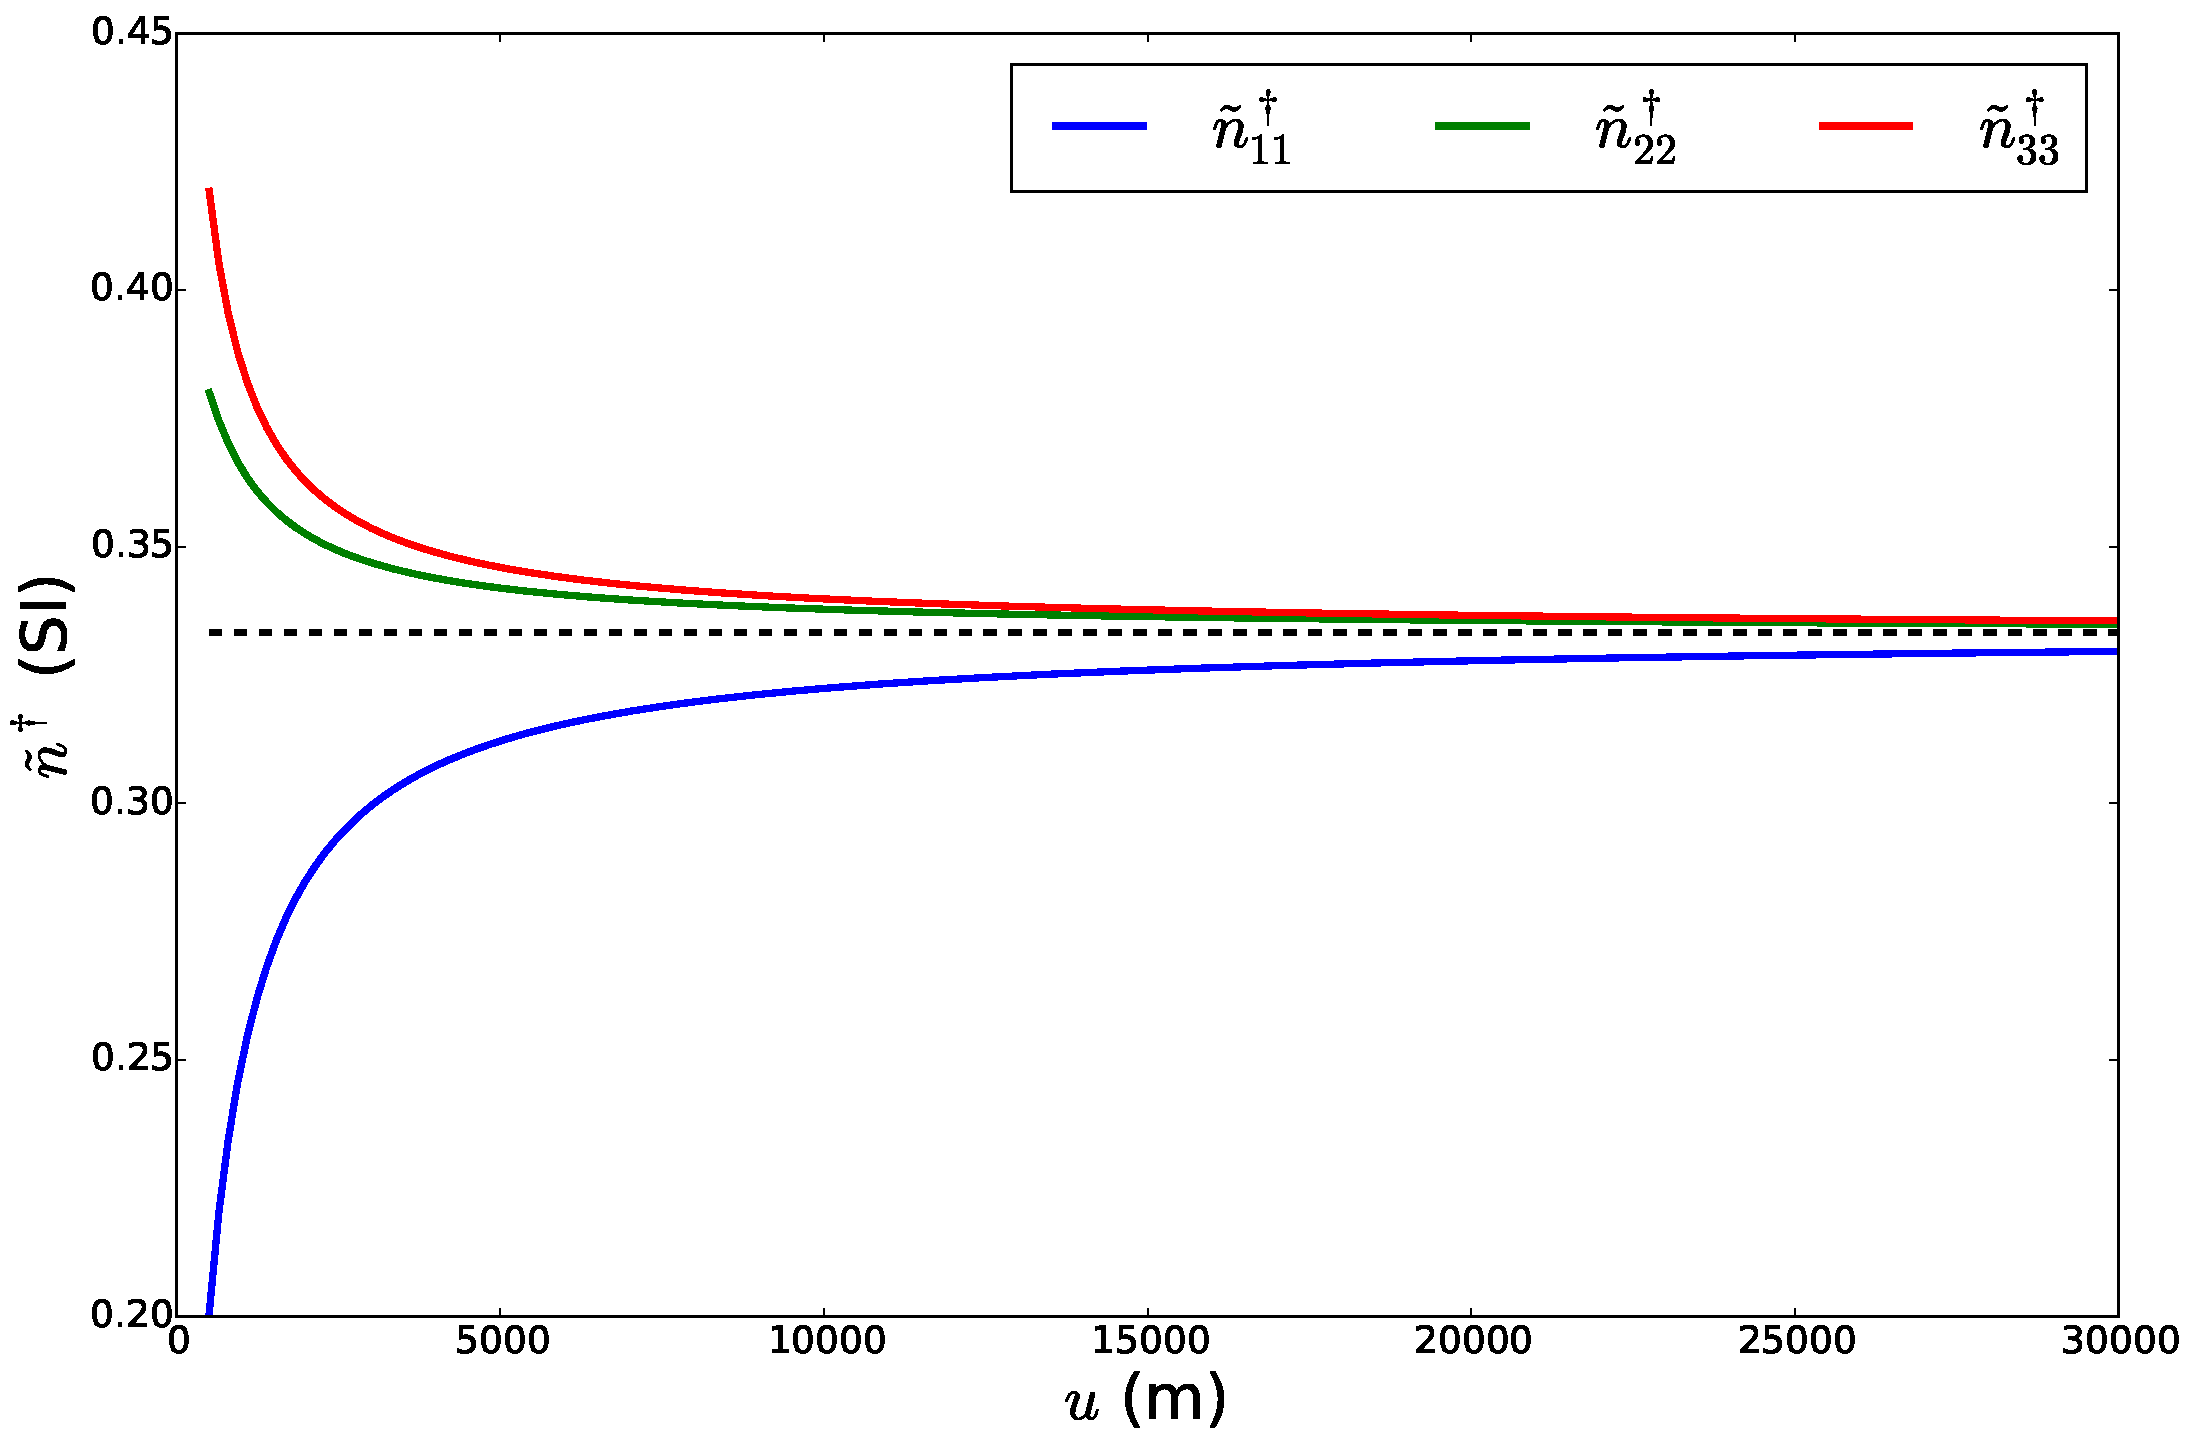
\includegraphics[width=15cm,height=10cm]{figures/test_n_triaxial}
	\caption[Comparação dos fatores de desmagnetização
	$\tilde{n}^{\dagger}_{11}$ (azul), $\tilde{n}^{\dagger}_{22}$ (verde) e $\tilde{n}^{\dagger}_{33}$ (vermelho) de um elipsoide triaxial originalmente com semi-eixos 500, 100 e 50 metros, com um fator $500 \le u \ge 30000$, somando, simultaneamente, todos os semi-eixos. Os fatores de desmagnetização foram calculados pelas Eq. \ref{eq:n-tilde-dagger-11-triaxial}, \ref{eq:n-tilde-dagger-22-triaxial} e \ref{eq:n-tilde-dagger-33-triaxial}.]{Comparação dos fatores de desmagnetização
		$\tilde{n}^{\dagger}_{11}$ (azul), $\tilde{n}^{\dagger}_{22}$ (verde) e $\tilde{n}^{\dagger}_{33}$ (vermelho) de um elipsoide triaxial originalmente com semi-eixos 500, 100 e 50 metros, com um fator $500 \le u \ge 30000$, somando, simultaneamente, todos os semi-eixos. Os fatores de desmagnetização foram calculados pelas Eq. \ref{eq:n-tilde-dagger-11-triaxial}, \ref{eq:n-tilde-dagger-22-triaxial} e \ref{eq:n-tilde-dagger-33-triaxial}.}
	\label{fig:n_triaxial}
\end{figure}

Na Figura \ref{fig:n_prolato} observamos o mesmo comportamento no caso triaxial para o caso do elipsoide prolato. Simulamos 200 elipsoides prolatos com semi-eixos $a=m\, b_0$ e $b=b_0$, em que $b_0=100$ m e $1,1 \le m \ge 100$ m. Calculamos seus fatores de desmagnetização $\tilde{n}^{\dagger}_{11}$ e $\tilde{n}^{\dagger}_{22}$ pelas Eqs. \ref{eq:n-tilde-dagger-11-prolate}, \ref{eq:n-tilde-dagger-22-prolate}.
Neste gráfico no eixo horizontal é feita a relação entre os semi-eixos $a$ e $b$ ($m$) onde aumenta-se a valor do semi-eixo maior e mantém o semi-eixo menor constante. No começo, quando os semi-eixos estão próximos, os elementos tendem à $1/3$ e se afastam conforme $a$ é muito maior que $b$.
\newpage

\begin{figure}[hbt!]
	\centering 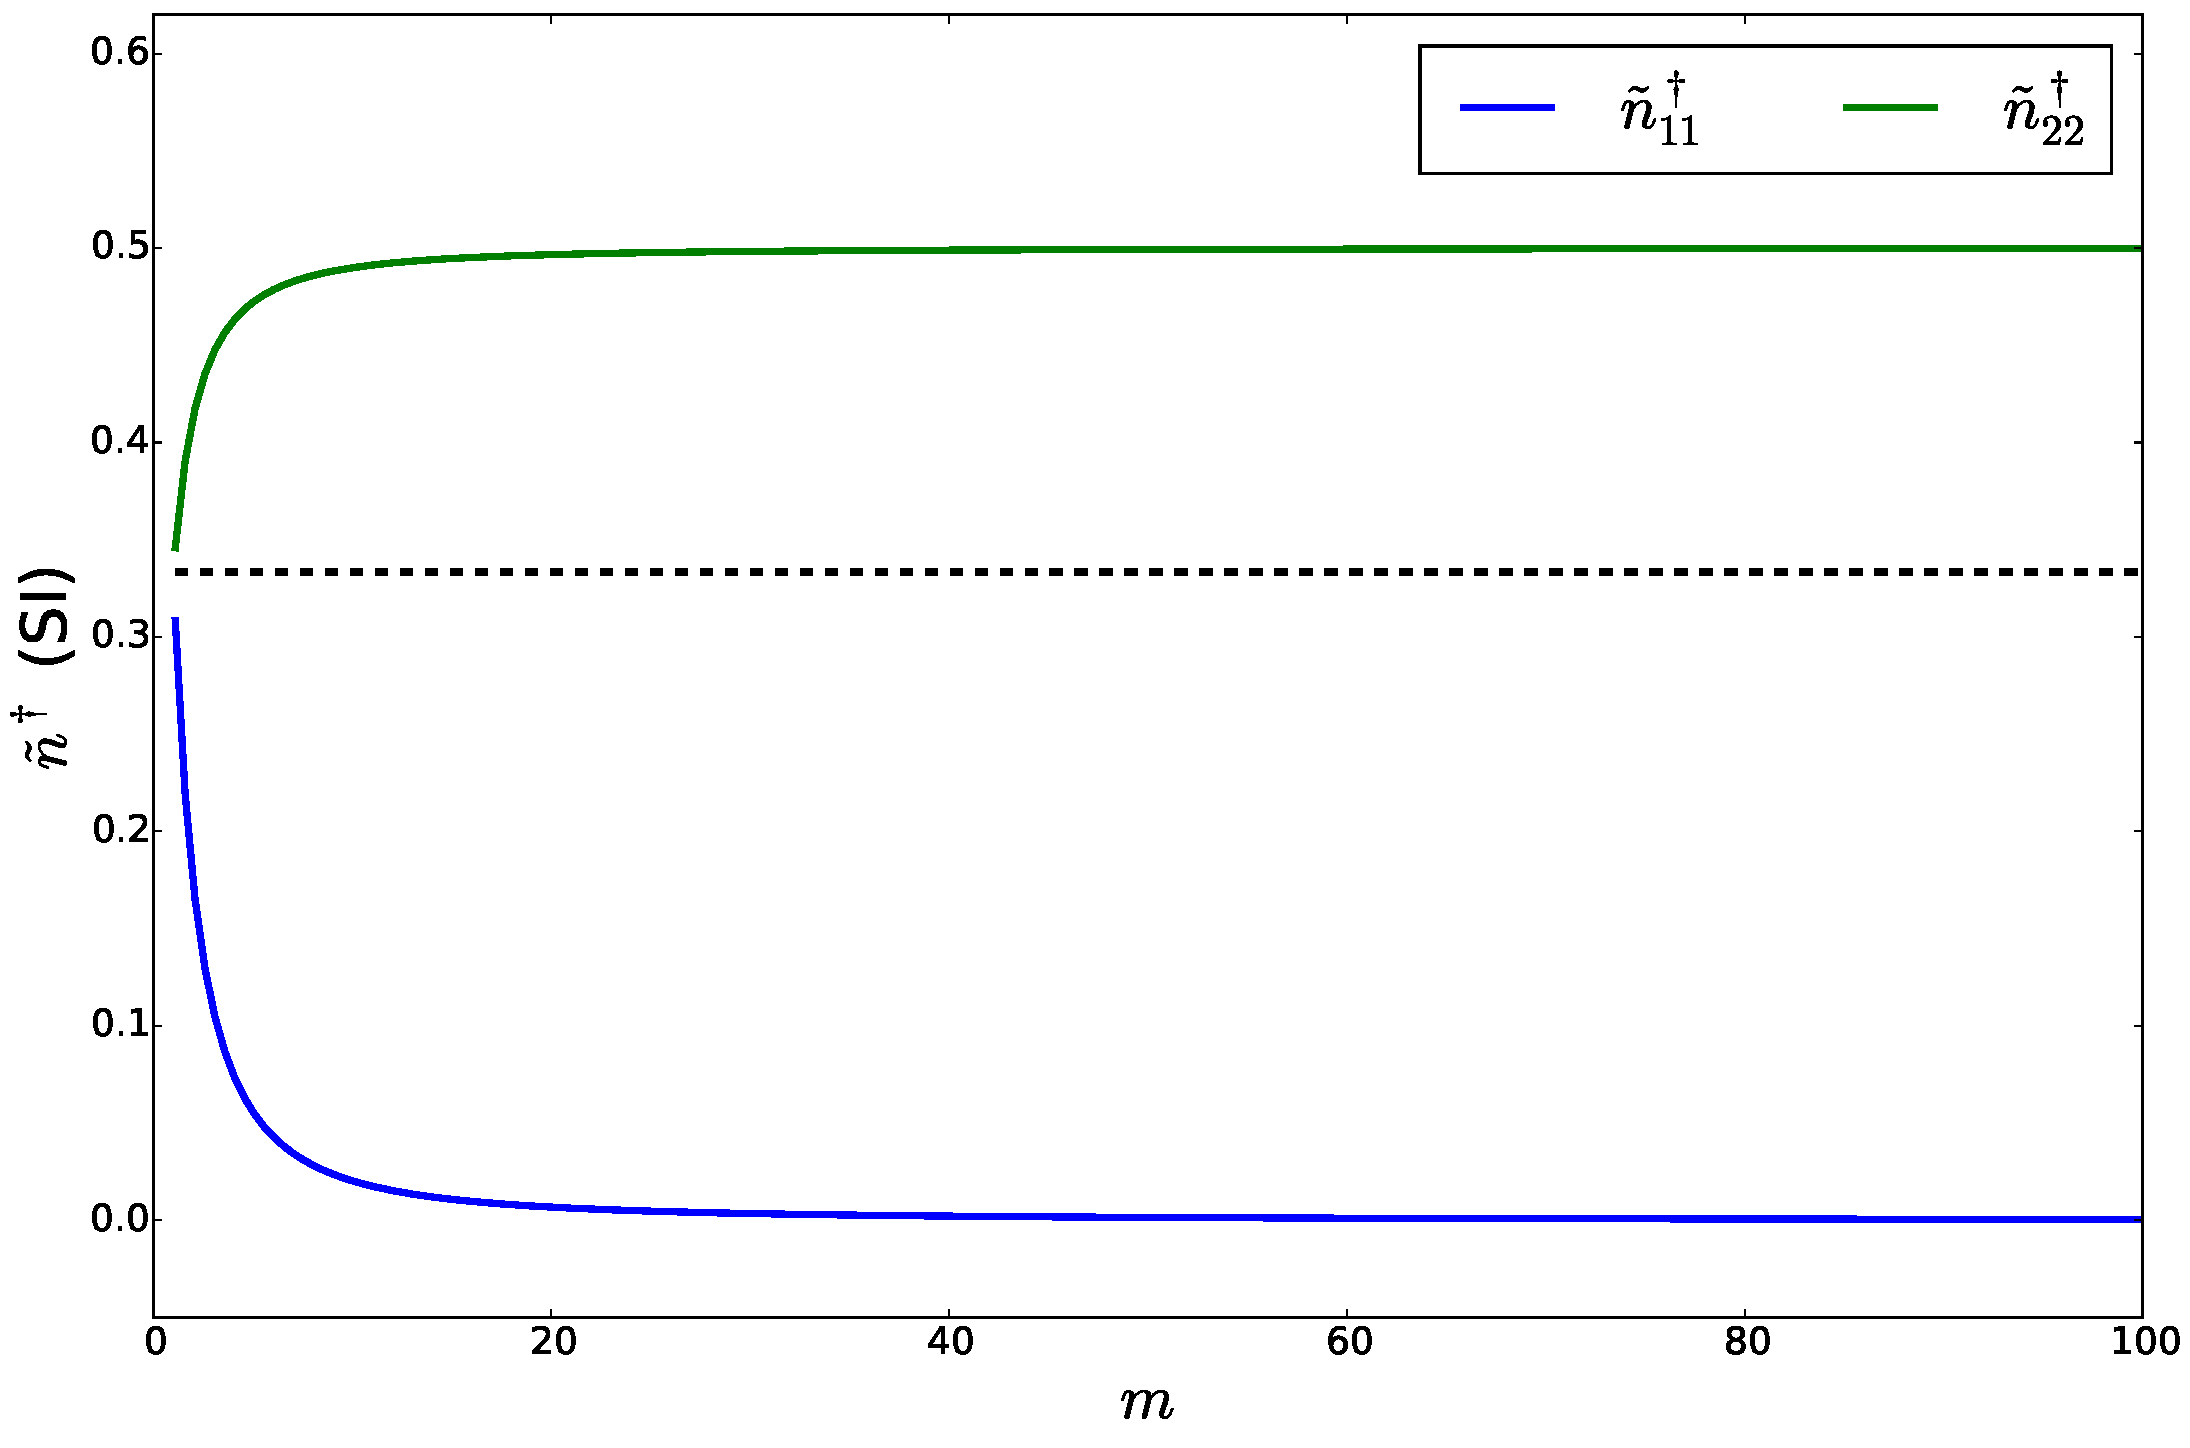
\includegraphics[width=15cm,height=10cm]{figures/test_n_prolate}
	\caption[Comparação dos fatores de desmagnetização
	$\tilde{n}^{\dagger}_{11}$ (azul) e $\tilde{n}^{\dagger}_{22}$ (verde) de um elipsoide prolato originalmente com semi-eixo $b_0=100$ m, com um fator $1,1 \le m \ge 100$, que aumenta a valor do semi-eixo maior e mantém o semi-eixo menor constante. Os fatores de desmagnetização foram calculados pelas Eq. \ref{eq:n-tilde-dagger-11-prolate}, \ref{eq:n-tilde-dagger-22-prolate}.]{Comparação dos fatores de desmagnetização
		$\tilde{n}^{\dagger}_{11}$ (azul) e $\tilde{n}^{\dagger}_{22}$ (verde) de um elipsoide prolato originalmente com semi-eixo $b_0=100$ m, com um fator $1,1 \le m \ge 100$, que aumenta a valor do semi-eixo maior e mantém o semi-eixo menor constante. Os fatores de desmagnetização foram calculados pelas Eq. \ref{eq:n-tilde-dagger-11-prolate}, \ref{eq:n-tilde-dagger-22-prolate}.}
	\label{fig:n_prolato}
\end{figure}

De forma similar, simulamos 200 elipsoides oblatos com semi-eixos $a=m\, b_0$ e $b=b_0$, em que $b_0=1000$ m e $0,05 \le m \ge 1$. Calculamos seus fatores de desmagnetização $\tilde{n}^{\dagger}_{11}$ e $\tilde{n}^{\dagger}_{22}$ pelas Eqs. \ref{eq:n-tilde-dagger-11-oblate}, \ref{eq:n-tilde-dagger-22-oblate}. Na figura \ref{fig:n_oblato} temos o resultado dessa simulação. Lembremos que no caso do elipsoide oblato $a$ é o semi-eixo menor e $b$ o semi-eixo maior. No começo, quando os semi-eixos possuem valores discrepantes, os elementos estão afastados para $b$ muito maior que $a$ e tendem à $1/3$ conforme se aproximam.
\newpage

\begin{figure}[hbt!]
	\centering 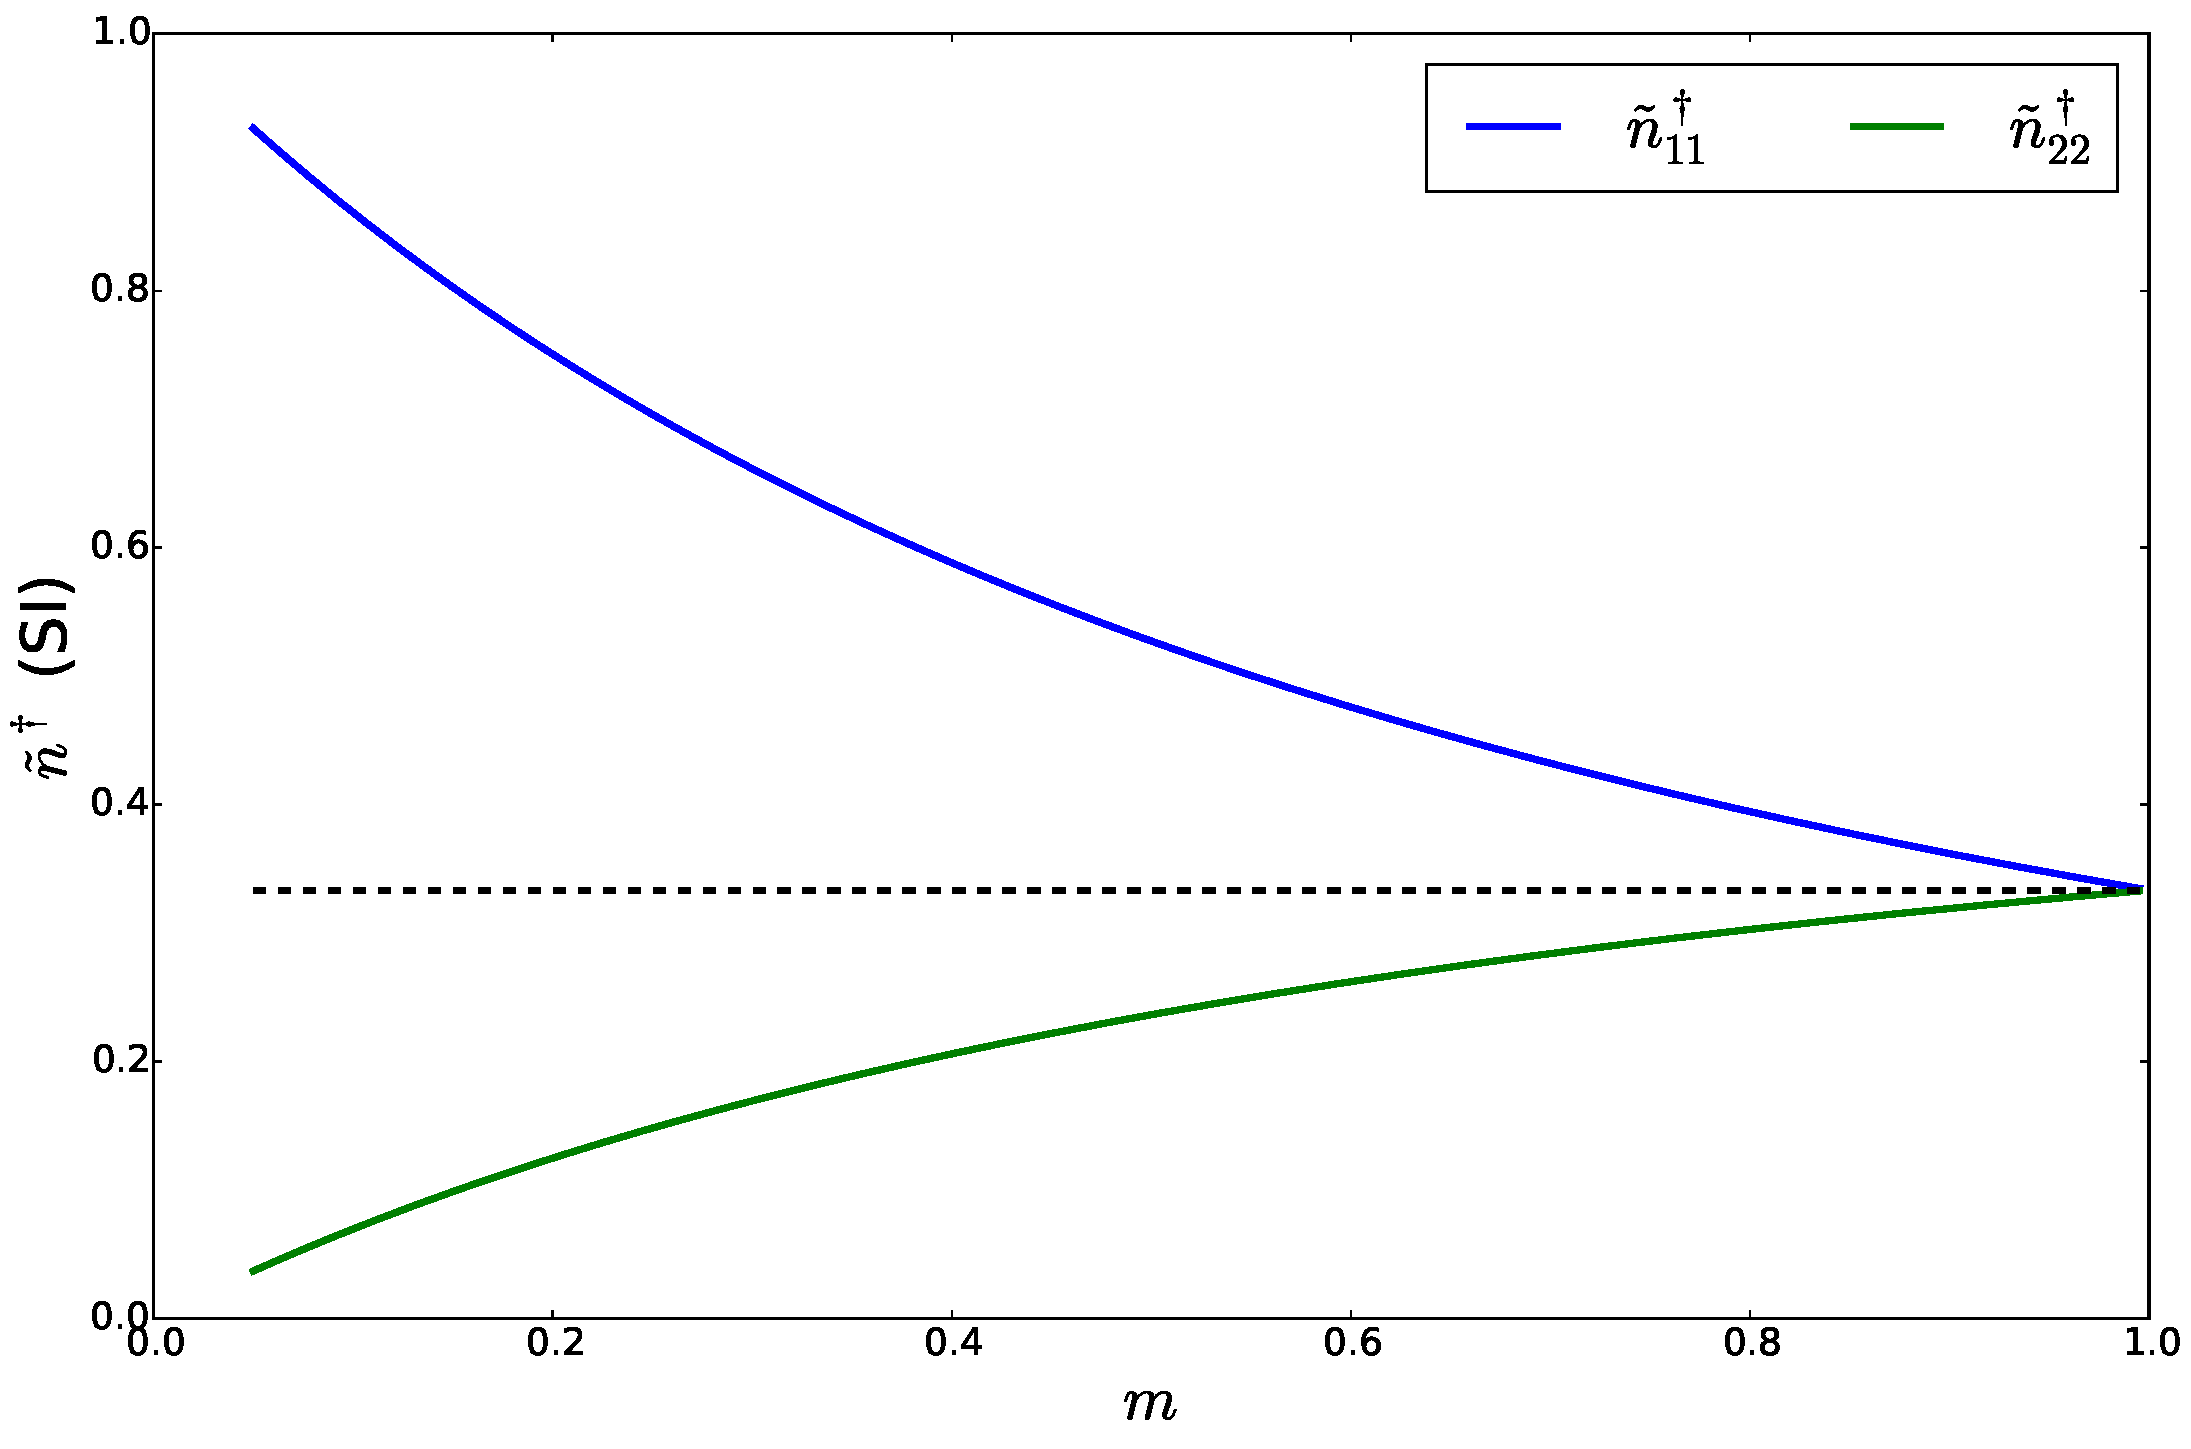
\includegraphics[width=15cm,height=10cm]{figures/test_n_oblate}
	\caption[Comparação dos fatores de desmagnetização
	$\tilde{n}^{\dagger}_{11}$ (azul) e $\tilde{n}^{\dagger}_{22}$ (verde) de um elipsoide oblato originalmente com semi-eixo $b_0=1000$ m, com um fator $0,05 \le m \ge 1$, que aumenta a valor do semi-eixo menor e mantém o semi-eixo maior constante. Os fatores de desmagnetização foram calculados pelas Eq. \ref{eq:n-tilde-dagger-11-oblate}, \ref{eq:n-tilde-dagger-22-oblate}.]{Comparação dos fatores de desmagnetização
		$\tilde{n}^{\dagger}_{11}$ (azul) e $\tilde{n}^{\dagger}_{22}$ (verde) de um elipsoide oblato originalmente com semi-eixo $b_0=1000$ m, com um fator $0,05 \le m \ge 1$, que aumenta a valor do semi-eixo menor e mantém o semi-eixo maior constante. Os fatores de desmagnetização foram calculados pelas Eq. \ref{eq:n-tilde-dagger-11-oblate}, \ref{eq:n-tilde-dagger-22-oblate}.}
	\label{fig:n_oblato}
\end{figure}

Através destes gráficos é possível observar como os fatores de desmagnetização possuem valor menor, quanto maior o semi-eixo do elipsoide. De fato há uma relação: $\tilde{n}^{\dagger}_{11}$ está relacionado com o semi-eixo maior, $\tilde{n}^{\dagger}_{22}$ com o semi-eixo intermediário e $\tilde{n}^{\dagger}_{33}$ com o semi-eixo menor. Fisicamente, isto significa que há a tendência, do elipsoide se desmagnetizar com maior intensidade na direção dos seus semi-eixos menores.

\section{Comparações entre a $\Delta T (\mathbf{r})$ produzida por modelos elipsoidais similares}

A Figura \ref{fig:triaxial_sphere} mostra as anomalias de campo total $\Delta T (\mathbf{r})$ produzidas pelo elipsoide triaxial definido na Tabela 4.5 e por uma esfera. Os dados produzidos pela esfera foram calculados com o pacote \textit{Fatiando a Terra}.
\newpage

\begin{table}[h!]
	\begin{center}
		\begin{tabular}{lc}
			
			&  \\
			& \\
			& \\
			& \\
			& \\
			& \\
			& \\
			& \\
			& \\
			& \\
			& \\
			& \\
			& \\
		\end{tabular}
	\end{center}
\end{table}

\begin{table}[h!]
	\begin{center}
		\begin{tabular}{|l|c|c|}
			\hline
			\textbf{Parâmetro}  & \textbf{Valor}  & \textbf{Unidade}\\
			\hline 
			$a$, $b$, $c$   & 500.0001, 500.0, 499.9999   & m\\
			\hline
			\textit{strike}   & $0$ & $^{\circ}$\\
			\hline
			\textit{dip}    & $0$ & $^{\circ}$\\
			\hline
			\textit{rake}   & $0$  & $^{\circ}$\\
			\hline
			$x_c $   & 0  & m\\
			\hline          
			$y_c $   & 0  & m\\
			\hline                
			$z_c $   & 1000  & m\\
			\hline
			$\mathbf{M}_{R}$*  & 100, $25$, $40$  & $A/m$, $^{\circ}$, $^{\circ}$\\
			\hline
			$\mathbf{B}_{0}$*    & 1, $50$, $20$ & $nT$, $^{\circ}$, $^{\circ}$\\
			\hline
			$k_{1}$, $k_{2}$, $k_{3}$   & 0,1, 0,1, 0,1 & SI, SI, SI \\
			\hline
			Orientação das colunas da matriz $\mathbf{U}$**   & $0$, $90$, $90$  & $^{\circ}$, $^{\circ}$, $^{\circ}$\\
			\hline
		\end{tabular}
		\caption{Parâmetros do elipsoide triaxial modelado. *Valores de intensidade, inclinação e declinação respectivamente. **Ângulo de \textit{strike} , \textit{dip}  e \textit{rake} , respectivamente, para calcular os vetores unitários $\mathbf{u}_{1}$, $\mathbf{u}_{2}$, $\mathbf{u}_{3}$ por meio das Eqs. \ref{eq:v1_triaxial_prolate}, \ref{eq:v2_triaxial_prolate} e \ref{eq:v3_triaxial_prolate}.}
	\end{center}
	\label{tab:triaxial_sphere}
\end{table}

\begin{table}[h!]
	\begin{center}
		\begin{tabular}{lc}
			
			&  \\
			& \\
			& \\
			& \\
			& \\
			& \\
			& \\
			& \\
			& \\
			& \\
			& \\
			& \\
				
		\end{tabular}
	\end{center}
\end{table}

\begin{figure}[hbt!]
	\centering 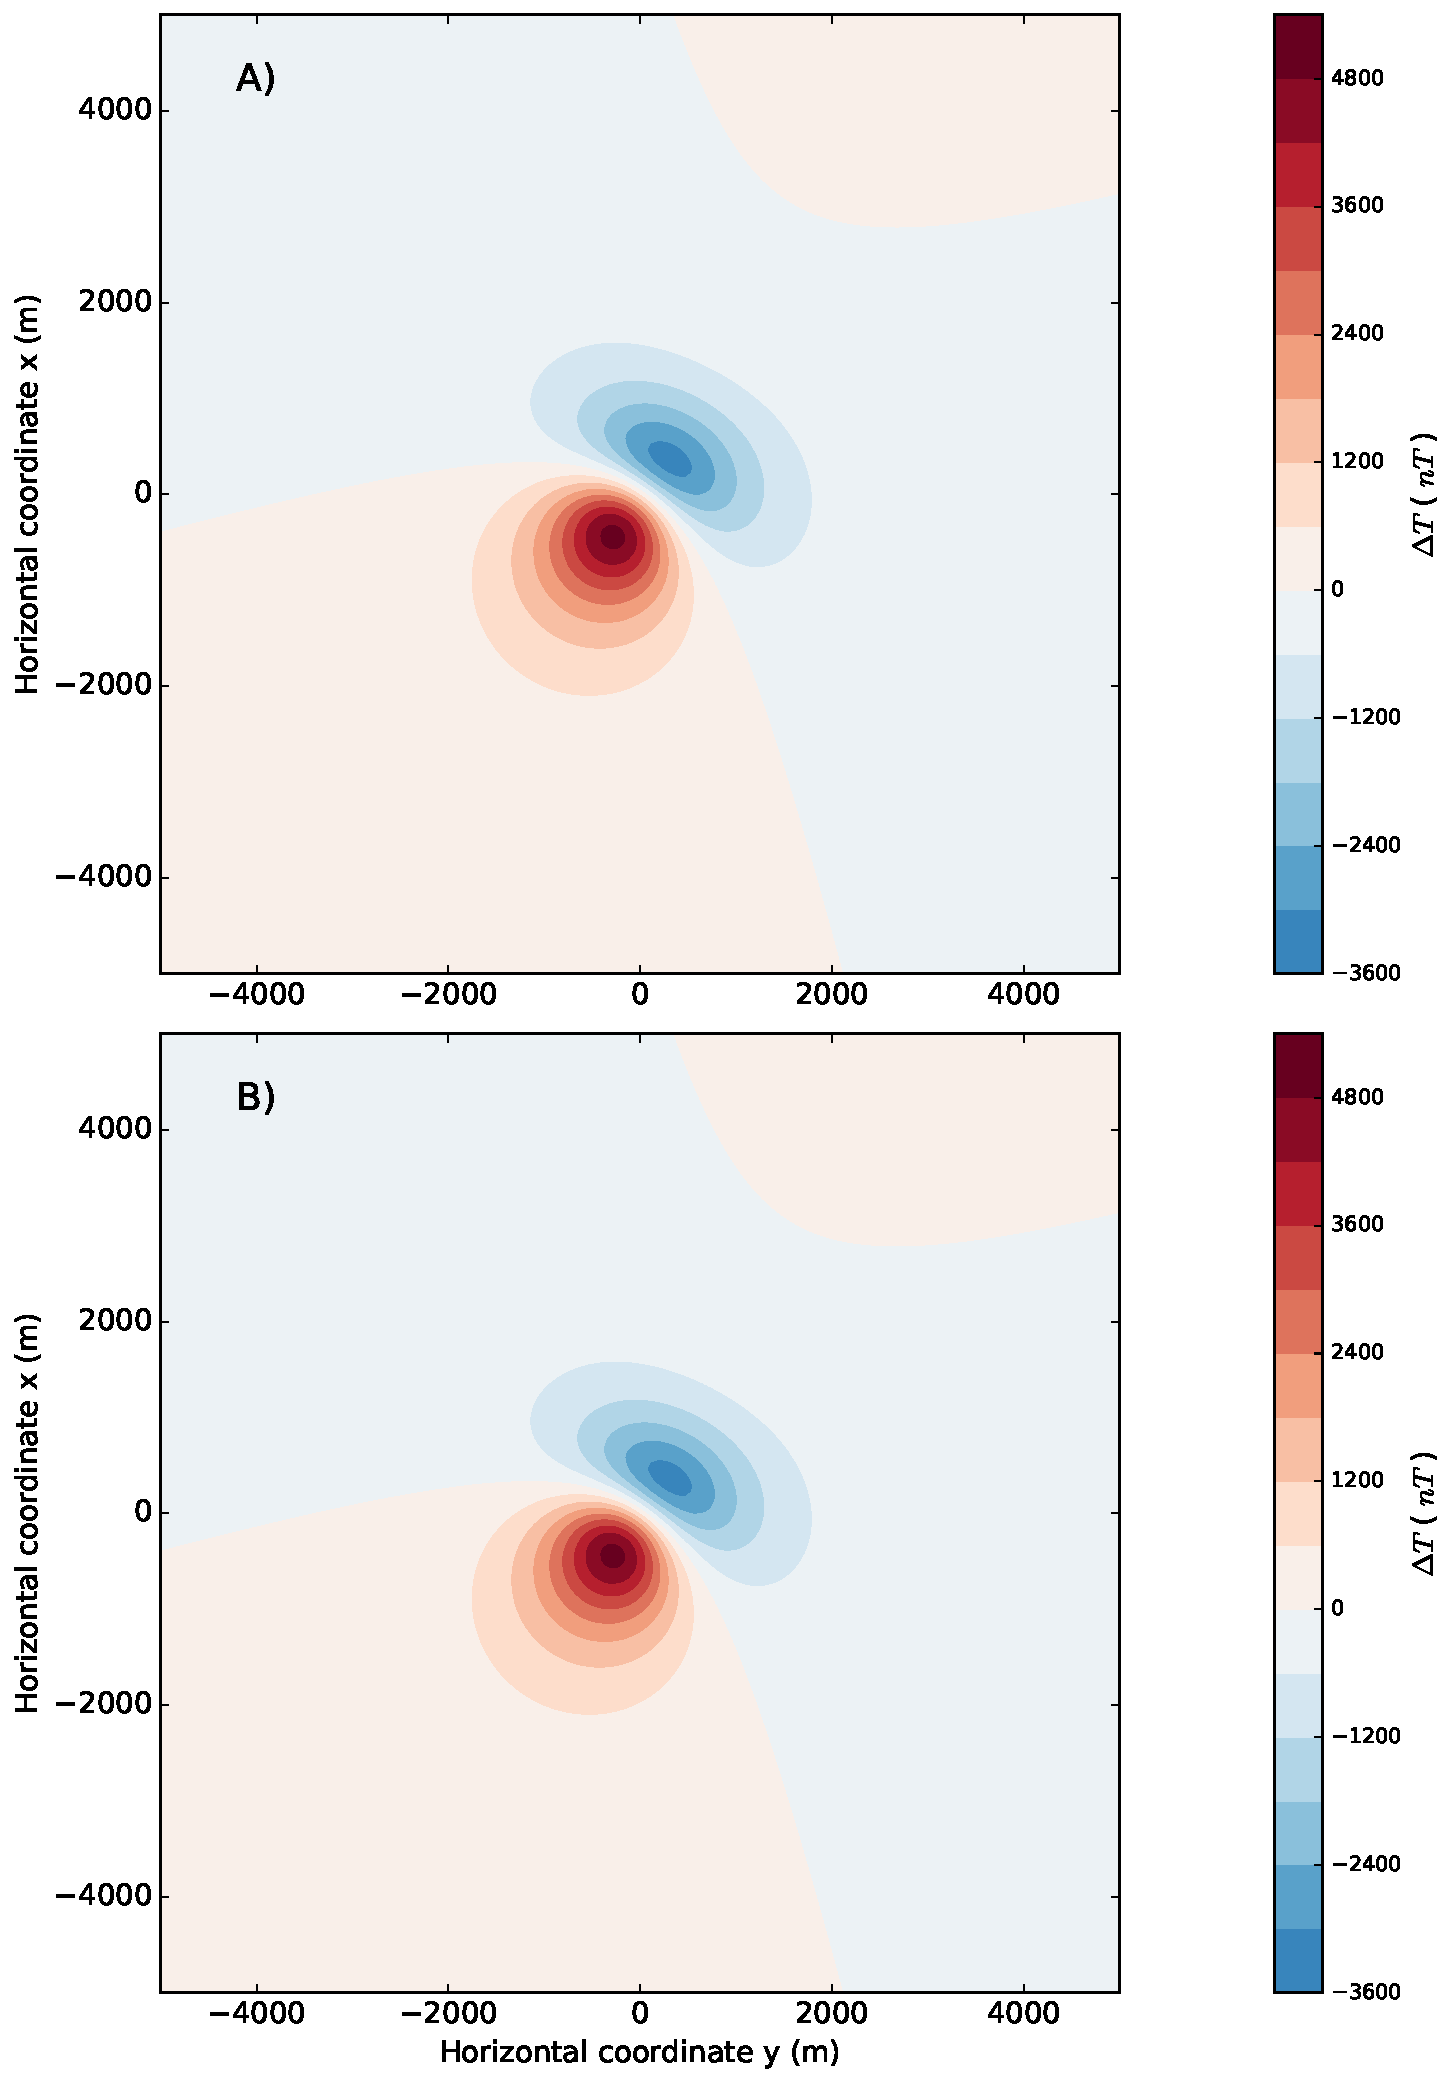
\includegraphics[width=14.5 cm,height=22 cm]{figures/ellipsoid_triaxial_sphere}
	\caption[Comparação entre a anomalia de campo total $\Delta T (\mathbf{r})$ (Eq. \ref{eq:delta-T-tilde-approx}) produzida (A) pelo elipsoide triaxial definido na Tabela 4.5 e (B) por uma esfera com centro em $(0, 0, 1000)$ e raio $500$ m. Os dois corpos sintéticos possuem a mesma magnetização $\mathbf{M}$ (Eq. \ref{eq:M-p-remanence}). A anomalia produzida pela esfera foi calculada utilizando-se o pacote Fatiando a Terra. Os dados estão calculados em uma malha regular de $200 \times 200$ pontos, no plano horizontal $z = 0$ m.]{Comparação entre a anomalia de campo total $\Delta T (\mathbf{r})$ (Eq. \ref{eq:delta-T-tilde-approx}) produzida (A) pelo elipsoide triaxial definido na Tabela 4.5 e (B) por uma esfera com centro em $(0, 0, 0)$ e raio $500$ m. Os dois corpos sintéticos possuem a mesma magnetização $\mathbf{M}$ (Eq. \ref{eq:M-p-remanence}). A anomalia produzida pela esfera foi calculada utilizando-se o pacote Fatiando a Terra. Os dados estão calculados em uma malha regular de $200 \times 200$ pontos, no plano horizontal $z = 0$ m.}
	\label{fig:triaxial_sphere}
\end{figure}

Tal como esperado, as anomalias de campo total produzidas pelo elipsoide triaxial (Fig. \ref{fig:triaxial_sphere}A) e pela esfera (Fig. \ref{fig:triaxial_sphere}B) são muito próximas. As diferenças máximas ocorrem nas regiões de máximo/mínimo das anomalias e atingem um valor absoluto de $\sim 0.000349$ nT. Estes resultados representam uma validação numérica das rotinas desenvolvidas neste trabalho para calcular a anomalia de campo total produzida por elipsoides triaxiais.

As Figuras \ref{fig:triaxial_prolate}A e \ref{fig:triaxial_prolate}B mostram as anomalias de campo total $\Delta T (\mathbf{r})$ (Eq. \ref{eq:delta-T-tilde-approx}) produzidas, respectivamente, pelo elipsoide triaxial definido na Tabela 4.6 e pelo elipsoide prolato definido na Tabela 4.7. As maiores diferenças ocorrem na região de máximo/minimo das anomalias e atingem um valor absoluto de $\sim 0.003788$ nT. Similarmente, as Figuras \ref{fig:triaxial_oblate}A e \ref{fig:triaxial_oblate}B mostram as anomalias de campo total $\Delta T (\mathbf{r})$ (Eq. \ref{eq:delta-T-tilde-approx}) produzidas, respectivamente, pelo elipsoide triaxial definido na Tabela 4.8 e pelo elipsoide oblato definido na Tabela 4.9. As maiores diferenças ocorrem na região de máximo/minimo das anomalias e atingem um valor absoluto de $\sim 46.71$ nT, o que representa cerca de $0,5\%$ do valor máximo da anomalia apresentada nesta simulação. Estes resultados servem como validação numérica e mostram a consistência entre as rotinas desenvolvidas neste trabalho.

\begin{table}[h!]
	\begin{center}
		\begin{tabular}{|l|c|c|}
			\hline
			\textbf{Parâmetro}  & \textbf{Valor}  & \textbf{Unidade} \\
			\hline 
			$a$, $b$, $c$  & 500, 100, 99.99 & m\\
			\hline
			\textit{strike}   & $90$ & $^{\circ}$\\
			\hline
			\textit{dip}    & $45$ & $^{\circ}$\\
			\hline
			\textit{rake}   & $0$  & $^{\circ}$\\
			\hline
			$x_c$   & 0 & m \\
			\hline          
			$y_c$   & 0  & m\\
			\hline                
			$z_c$   & 1000  & m\\
			\hline
			$\mathbf{M}_{R}$*  & 100, $90$, $0$  & $A/m$, $^{\circ}$, $^{\circ}$\\
			\hline
			$\mathbf{B}_{0}$*    & 60000, $50$, $20$ & $nT$, $^{\circ}$, $^{\circ}$\\
			\hline
			$k_{1}$, $k_{2}$, $k_{3}$   & 0,2, 0,1, 0,05  & SI, SI, SI\\
			\hline
			Orientação das colunas da matriz $\mathbf{U}$**   & $0$, $90$, $90$  & $^{\circ}$, $^{\circ}$, $^{\circ}$\\
			\hline
		\end{tabular}
		\caption{Parâmetros do elipsoide triaxial modelado. *Valores de intensidade, inclinação e declinação respectivamente. **Ângulo de \textit{strike} , \textit{dip}  e \textit{rake} , respectivamente, para calcular os vetores unitários $\mathbf{u}_{1}$, $\mathbf{u}_{2}$, $\mathbf{u}_{3}$ por meio das Eqs. \ref{eq:v1_triaxial_prolate}, \ref{eq:v2_triaxial_prolate} e \ref{eq:v3_triaxial_prolate}.}
	\end{center}
	\label{tab:triaxial_prolate1}
\end{table}

\vspace{2cm}

\begin{table}[h!]
	\begin{center}
		\begin{tabular}{|l|c|c|}
			\hline
			\textbf{Parâmetro}  & \textbf{Valor}  & \textbf{Unidade}\\
			\hline 
			$a$, $b$  & 500, 100 & m\\
			\hline
			\textit{strike}   & $90$ & $^{\circ}$\\
			\hline
			\textit{dip}    & $45$ & $^{\circ}$\\
			\hline
			\textit{rake}   & $0$  & $^{\circ}$\\
			\hline
			$x_c$   & 0  & m\\
			\hline          
			$y_c$   & 0  & m\\
			\hline                
			$z_c$  & 1000  & m\\
			\hline
			$\mathbf{M}_{R}$*  & 100, $90$, $0$  & $A/m$, $^{\circ}$, $^{\circ}$\\
			\hline
			$\mathbf{B}_{0}$*    & 60000, $50$, $20$ & $nT$, $^{\circ}$, $^{\circ}$\\
			\hline
			$k_{1}$, $k_{2}$, $k_{3}$   & 0,2, 0,1, 0,05  & SI, SI, SI\\
			\hline
			Orientação das colunas da matriz $\mathbf{U}$**   & $0$, $90$, $90$  & $^{\circ}$, $^{\circ}$, $^{\circ}$\\
			\hline
		\end{tabular}
		\caption{Parâmetros do elipsoide prolato modelado. *Valores de intensidade, inclinação e declinação respectivamente. **Ângulo de \textit{strike} , \textit{dip}  e \textit{rake} , respectivamente, para calcular os vetores unitários $\mathbf{u}_{1}$, $\mathbf{u}_{2}$, $\mathbf{u}_{3}$ por meio das Eqs. \ref{eq:v1_triaxial_prolate}, \ref{eq:v2_triaxial_prolate} e \ref{eq:v3_triaxial_prolate}.}
	\end{center}
	\label{tab:triaxial_prolate2}
\end{table}

\begin{figure}[hbt!]
	\centering \includegraphics[width=14.5 cm,height=22 cm]{figures/ellipsoid_triaxial_prolate}
	\caption[Comparação entre a anomalia de campo total $\Delta T (\mathbf{r})$ (Eq. \ref{eq:delta-T-tilde-approx}) produzida (A) pelo elipsoide triaxial definido na Tabela 4.7 e (B) produzida pelo elipsoide prolato definido na Tabela 4.6.]{Comparação entre a anomalia de campo total $\Delta T (\mathbf{r})$ (Eq. \ref{eq:delta-T-tilde-approx}) produzida (A) pelo elipsoide triaxial definido na Tabela 4.6 e (B) produzida pelo elipsoide prolato definido na Tabela 4.7.}
	\label{fig:triaxial_prolate}
\end{figure}

\begin{table}[h!]
	\begin{center}
		\begin{tabular}{|l|c|c|}
			\hline
			\textbf{Parâmetro}  & \textbf{Valor} & \textbf{Unidade} \\
			\hline 
			$a$, $b$, $c$   & 500, 499.99, 499.98 & m\\
			\hline
			\textit{strike}   & $0$ & $^{\circ}$\\
			\hline
			\textit{dip}   & $0$ & $^{\circ}$\\
			\hline
			\textit{rake}   & $90$  & $^{\circ}$\\
			\hline
			$x_c$   & 0  & m\\
			\hline          
			$y_c$   & 0  & m\\
			\hline                
			$z_c$   & 1000 & m \\
			\hline
			$\mathbf{M}_{R}$*  & 100, $90$, $0$ & $A/m$, $^{\circ}$, $^{\circ}$ \\
			\hline
			$\mathbf{B}_{0}$*    & 60000, $50$, $20$ & $nT$, $^{\circ}$, $^{\circ}$ \\
			\hline
			$k_{1}$, $k_{2}$, $k_{3}$   & 0,1, 0,1, 0,1 & SI, SI, SI \\
			\hline
			Orientação das colunas da matriz $\mathbf{U}$**  & $0$, $90$, $90$ & $^{\circ}$, $^{\circ}$, $^{\circ}$ \\
			\hline
		\end{tabular}
		\caption{Parâmetros do elipsoide triaxial modelado. *Valores de intensidade, inclinação e declinação respectivamente. **Ângulo de \textit{strike} , \textit{dip}  e \textit{rake} , respectivamente, para calcular os vetores unitários $\mathbf{u}_{1}$, $\mathbf{u}_{2}$, $\mathbf{u}_{3}$ por meio das Eqs. \ref{eq:v1_triaxial_prolate}, \ref{eq:v2_triaxial_prolate} e \ref{eq:v3_triaxial_prolate}.}
	\end{center}
	\label{tab:triaxial_oblate1}
\end{table}

\vspace{2cm}

\begin{table}[h!]
	\begin{center}
		\begin{tabular}{|l|c|c|}
			\hline
			\textbf{Parâmetro}  & \textbf{Valor} & \textbf{Unidade} \\
			\hline 
			$a$, $b$   & 499,99, 500 & m\\
			\hline
			\textit{strike}   & $0$ & $^{\circ}$\\
			\hline
			\textit{dip}    & $0$ & $^{\circ}$\\
			\hline
			\textit{rake}   & $0$  & $^{\circ}$\\
			\hline
			$x_c$   & 0  & m\\
			\hline          
			$y_c$   & 0  & m\\
			\hline                
			$z_c$   & 1000  & m\\
			\hline
			$\mathbf{M}_{R}$*  & 100, $90$, $0$  & $A/m$, $^{\circ}$, $^{\circ}$\\
			\hline
			$\mathbf{B}_{0}$*    & 60000, $50$, $20$ & $nT$, $^{\circ}$, $^{\circ}$ \\
			\hline
			$k_{1}$, $k_{2}$, $k_{3}$   & 0,1, 0,1, 0,1 & SI, SI, SI \\
			\hline
			Orientação das colunas da matriz $\mathbf{U}$**   & $0$, $90$, $90$ & $^{\circ}$, $^{\circ}$, $^{\circ}$ \\
			\hline
		\end{tabular}
		\caption{Parâmetros do elipsoide oblato modelado. *Valores de intensidade, inclinação e declinação respectivamente. **Ângulo de \textit{strike} , \textit{dip}  e \textit{rake} , respectivamente, para calcular os vetores unitários $\mathbf{u}_{1}$, $\mathbf{u}_{2}$, $\mathbf{u}_{3}$ por meio das Eqs. \ref{eq:v1_oblate}, \ref{eq:v2_oblate} e \ref{eq:v3_oblate}.}
	\end{center}
	\label{tab:triaxial_oblate2}
\end{table}

\begin{figure}[hbt!]
	\centering \includegraphics[width=14.5 cm,height=22 cm]{figures/ellipsoid_triaxial_oblate}
	\caption[Comparação entre a anomalia de campo total $\Delta T (\mathbf{r})$ (Eq. \ref{eq:delta-T-tilde-approx}) produzida (A) pelo elipsoide triaxial definido na Tabela 4.8 e (B) produzida pelo elipsoide oblato definido na Tabela 4.9.]{Comparação entre a anomalia de campo total $\Delta T (\mathbf{r})$ (Eq. \ref{eq:delta-T-tilde-approx}) produzida (A) pelo elipsoide triaxial definido na Tabela 4.8 e (B) produzida pelo elipsoide oblato definido na Tabela 4.9.}
	\label{fig:triaxial_oblate}
\end{figure}

\section{Susceptibilidade}

Sabe-se que, na modelagem magnética de corpos geológicos com alta susceptibilidade, a desmagnetização é um fator muito importante. Nestes casos, negligenciar a desmagnetização e, consequentemente, utilizar a magnetização aproximada $\breve{\mathbf{M}}$ (Eq. \ref{eq:M-approx}) ao invés da magnetização $\mathbf{M}$ (Eq. \ref{eq:M-K-isotropic}) pode acarretar em erros de interpretação das anomalias em dados magnéticos. É comumente aceito na literatura que 0,1 SI é o valor de suscetibilidade isotrópica a partir do qual a desmagnetização deve ser considerada na modelagem ou seja, é o valor a partir do qual a magnetização aproximada $\breve{\mathbf{M}}$ (Eq. \ref{eq:M-approx}) não é considerada uma boa aproximação para a magnetização $\mathbf{M}$ (Eq. \ref{eq:M-K-isotropic}). Para suscetibilidades menores que 0,1 SI, considera-se que $\breve{\mathbf{M}}$ (Eq. \ref{eq:M-approx}) é uma boa aproximação para a magnetização resultante e que a parcela induzida tem a mesma direção do campo geomagnético local.

Para analisar o efeito da suscetibilidade na modelagem magnética, calculamos a magnetização resultante $\mathbf{M}$ (Eq. \ref{eq:M-K-isotropic}) do elipsoide triaxial definido na Tabela 4.10 para diferentes valores de suscetibilidade isotrópica $0,0001 \le \chi \ge 0,05$. A Figura \ref{fig:test_k_triaxial} mostra a inclinação (linha azul) e a declinação (linha verde) da magnetização resultante $\mathbf{M}$ (Eq. \ref{eq:M-K-isotropic}) em função da suscetibilidade $\chi$. A inclinação e a declinação do campo geomagnético local estão representadas, respectivamente, pelas linhas horizontais preta e vermelha. Nota-se que, para valores de suscetibilidade $\chi$ menores que 0,1 SI (linha preta vertical na Figura \ref{fig:test_k_triaxial}), a diferença entre a inclinação da magnetização resultante do elipsoide e do campo geomagnético local é menor que $-0,58$ graus. Já para a declinação, a diferença é menor que $0,85$ graus. Por outro lado, as diferenças na inclinação e declinação para valores de suscetibilidade $\chi = 0,5$ SI são próximos a $-2,71$ e $3,4$ graus, respectivamente. A linha vertical amarela na Figura \ref{fig:test_k_triaxial} mostra a suscetibilidade $\chi_{max}$ (Eq. \ref{eq:max-chi}) predita para que o erro relativo na magnetização resultante deste elipsoide seja menor ou igual a $\epsilon = 5 \%$. Neste caso, a suscetibilidade $\chi_{max}$ é menor que aquela comumente utilizada na literatura (0,1 SI) e as diferenças na inclinação e declinação são iguais a $-0,46$ e $0,68$ graus, respectivamente. Este resultado mostra que o valor de suscetibilidade isotrópica a partir do qual a desmagnetização deve ser considerada na modelagem pode ser escolhido de acordo com dois critérios: i) o conhecimento prévio do intérprete sobre a forma do corpo e ii) o máximo erro relativo $\epsilon$ permitido para a magnetização resultante.

\begin{table}[h!]
	\begin{center}
		\begin{tabular}{|l|c|c|}
			\hline
			\textbf{Parâmetro}  & \textbf{Valor} & \textbf{Unidade} \\
			\hline 
			$a$, $b$, $c$   & 500, 100, 50 & m\\
			\hline
			\textit{strike}   & $0$ & $^{\circ}$\\
			\hline
			\textit{dip}   & $0$ & $^{\circ}$\\
			\hline
			\textit{rake}   & $0$  & $^{\circ}$\\
			\hline
			$x_c$   & 0  & m\\
			\hline          
			$y_c$   & 0  & m\\
			\hline                
			$z_c$   & 500 & m \\
			\hline
			$\mathbf{M}_{R}$*  & 0, $0$, $0$ & $A/m$, $^{\circ}$, $^{\circ}$ \\
			\hline
			$\mathbf{B}_{0}$*    & 60000, $30$, $-15$ & $nT$, $^{\circ}$, $^{\circ}$ \\
			\hline
			$\chi$   & 0,0001-0,5 & SI, SI, SI \\
			\hline
			Orientação das colunas da matriz $\mathbf{U}$**  & $0$, $90$, $90$ & $^{\circ}$, $^{\circ}$, $^{\circ}$ \\
			\hline
		\end{tabular}
		\caption{Parâmetros do elipsoide triaxial modelado. *Valores de intensidade, inclinação e declinação respectivamente. **Ângulo de \textit{strike} , \textit{dip}  e \textit{rake} , respectivamente, para calcular os vetores unitários $\mathbf{u}_{1}$, $\mathbf{u}_{2}$, $\mathbf{u}_{3}$ por meio das Eqs. \ref{eq:v1_triaxial_prolate}, \ref{eq:v2_triaxial_prolate} e \ref{eq:v3_triaxial_prolate}.}
	\end{center}
	\label{tab:triaxial_k_iso}
\end{table}

\begin{figure}[hbt!]
	\centering 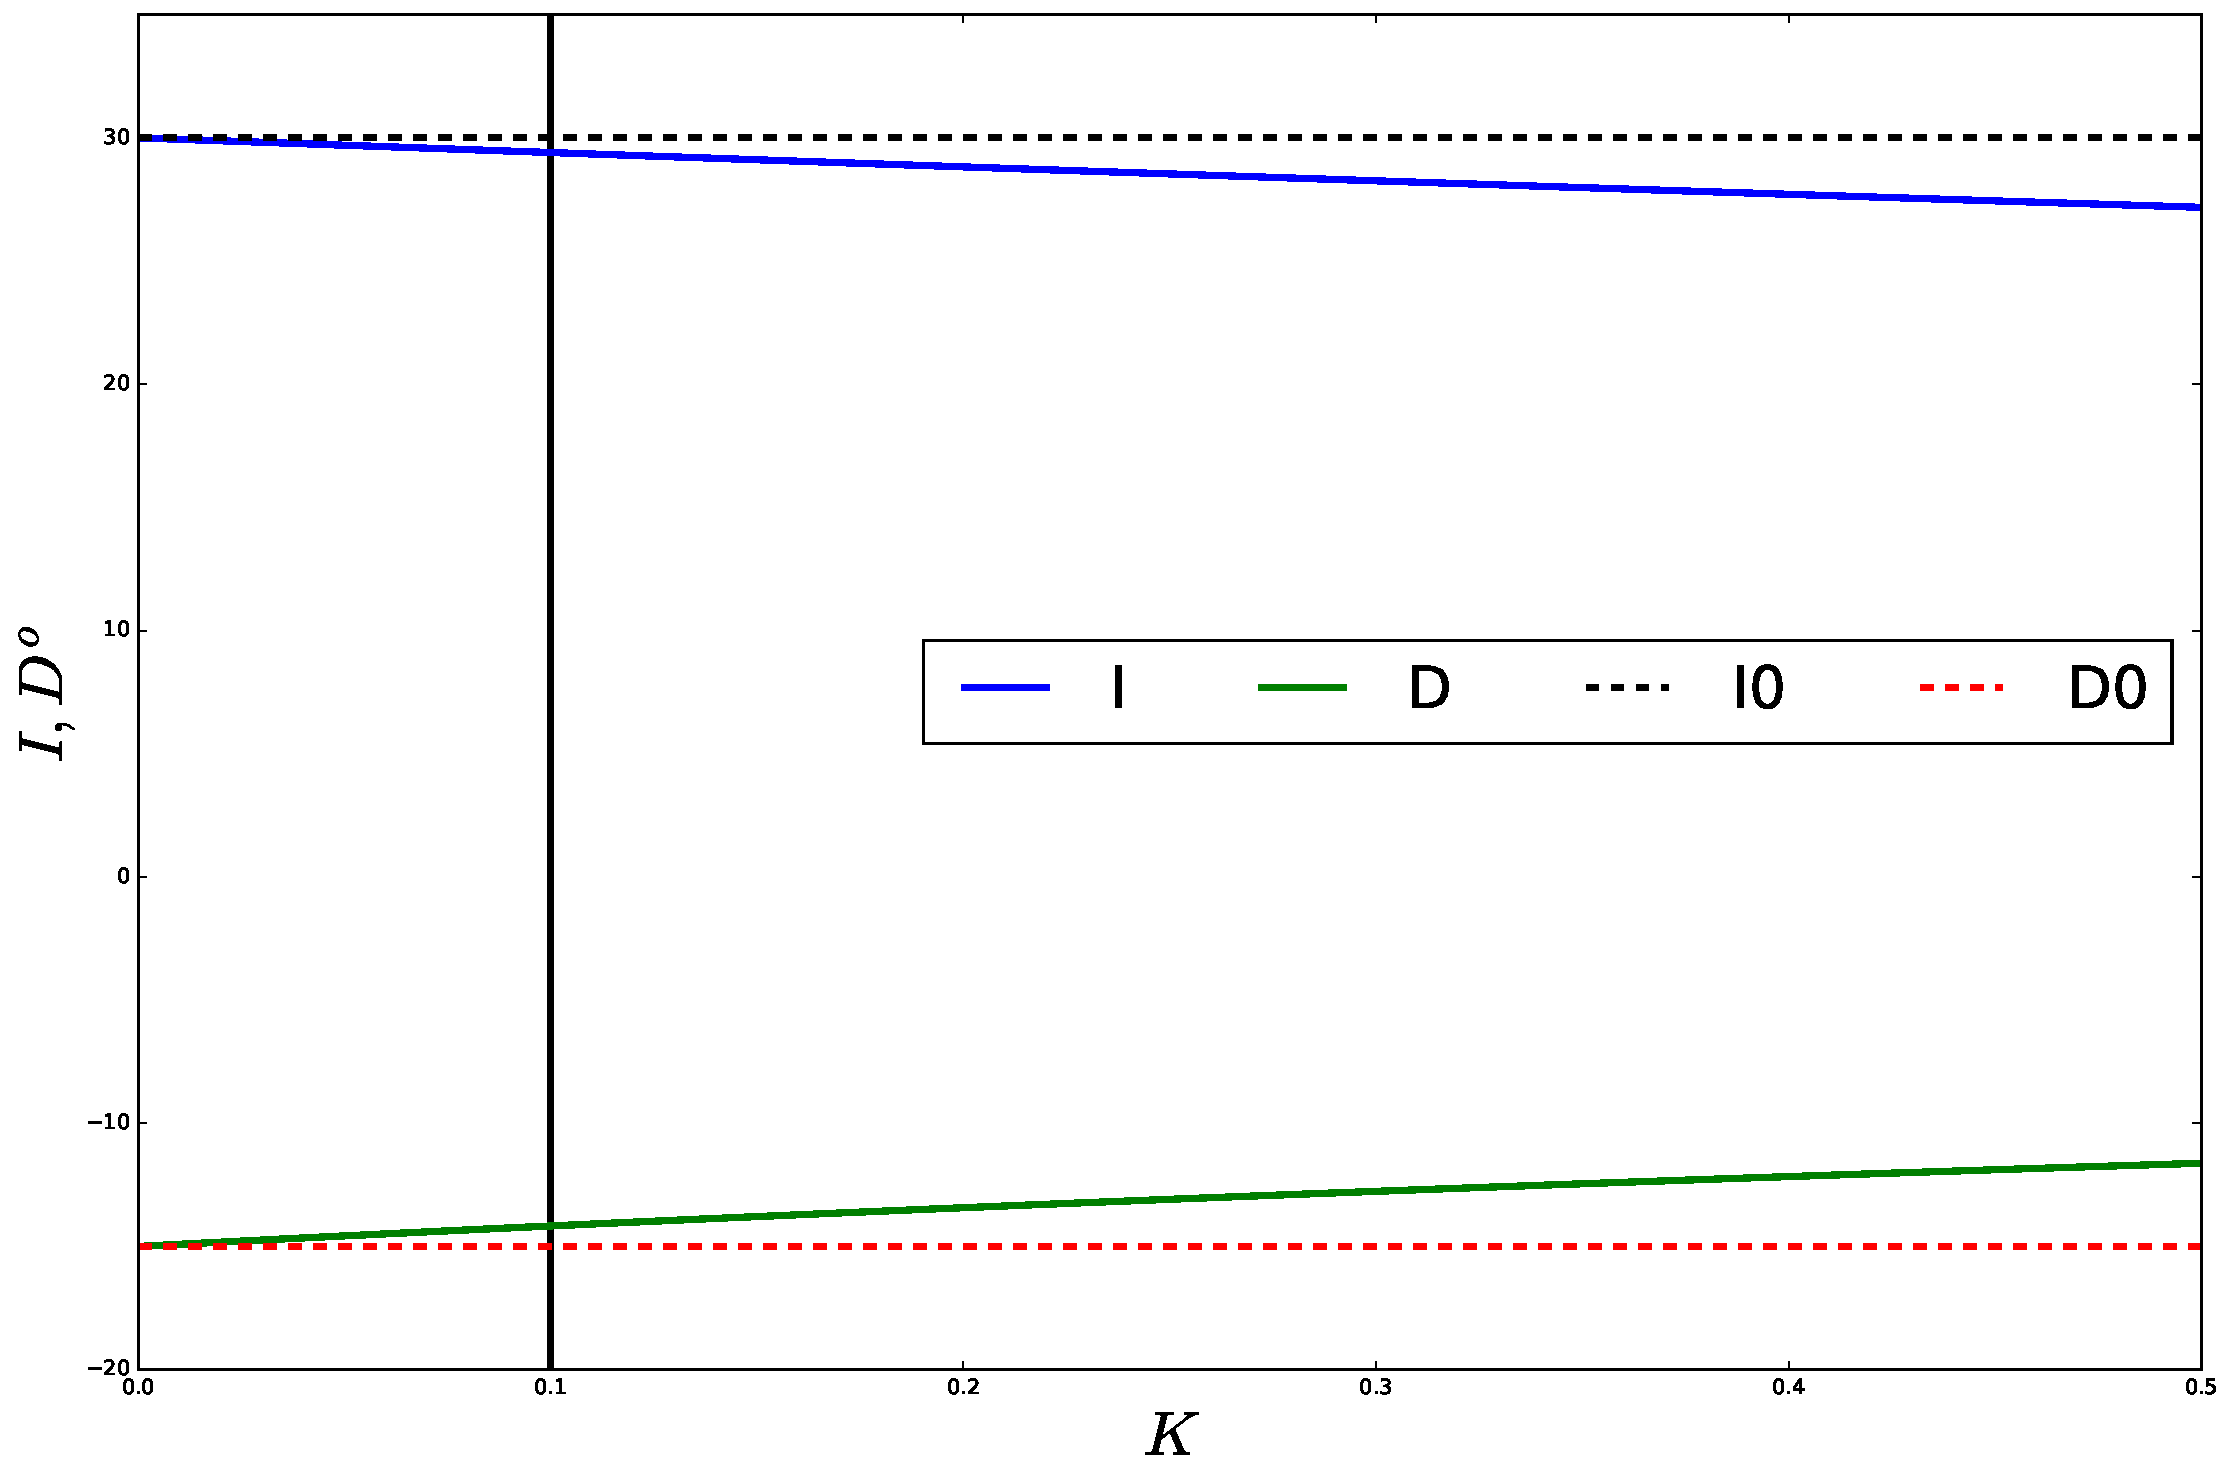
\includegraphics[width=15 cm,height=10 cm]{figures/test_k_triaxial}
	\caption[Efeito da susceptibilidade isotrópica $\chi$ na modelagem do elipsoide triaxial definido na Tabela 4.10. As linhas azul e verde representam, respectivamente, a inclinação $I$ e a declinação $D$ da magnetização resultante $\mathbf{M}$ (Eq. \ref{eq:M-K-isotropic}) deste elipsoide em função da suscetibilidade isotrópica $\chi$. As linhas horizontais preta e vermelha representam, respectivamente, a inclinação $I_{0}$ e a declinação $D_{0}$ do campo geomagnético local (Tabela 4.10). A linha vertical preta representa o valor de suscetibilidade isotrópica $\chi = 0,1$ SI, que é comumente aceito como o limite a partir do qual a desmagnetização deve ser considerada na modelagem. A linha vertical amarela representa a suscetibilidade isotrópica $\chi_{max}$ calculado com a Eq. \ref{eq:max-chi} para que o erro relativo na magnetização seja menor ou igual a $\epsilon = 5 \%$.]
	{Efeito da susceptibilidade isotrópica $\chi$ na modelagem do elipsoide triaxial definido na Tabela 4.10. As linhas azul e verde representam, respectivamente, a inclinação $I$ e a declinação $D$ da magnetização resultante $\mathbf{M}$ (Eq. \ref{eq:M-K-isotropic}) deste elipsoide em função da suscetibilidade isotrópica $\chi$. As linhas horizontais preta e vermelha representam, respectivamente, a inclinação $I_{0}$ e a declinação $D_{0}$ do campo geomagnético local (Tabela 4.10). A linha vertical preta representa o valor de suscetibilidade isotrópica $\chi = 0,1$ SI, que é comumente aceito como o limite a partir do qual a desmagnetização deve ser considerada na modelagem. A linha vertical amarela representa a suscetibilidade isotrópica $\chi_{max}$ calculado com a Eq. \ref{eq:max-chi} para que o erro relativo na magnetização seja menor ou igual a $\epsilon = 5 \%$.}
	\label{fig:test_k_triaxial}
\end{figure}